\documentclass[a4paper,10pt]{problems}

\begin{document}

\Header{Перебор с возвратом}

\begin{flushright}
Автор: Петр Калинин, основной текст: 2008\\
Этот документ можно распространять по лицензии\\
Creative Commons Attribution-ShareAlike 3.0 Unported (CC BY-SA 3.0)\\
Последнюю версию, а также исходный код для системы \LaTeX\\
можно скачать с \verb`https://github.com/petr-kalinin/progtexts`\\
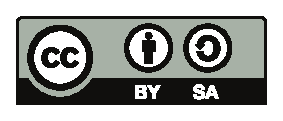
\includegraphics[width=2cm]{by-sa-corr.eps}
\end{flushright}

Перебор "--- довольно своеобразный метод решения задач. На серьезных олимпиадах 
задачи на перебор встречаются довольно редко, но все равно во многих задачах, в 
которых есть <<правильное>>, эффективное решение, перебор (хорошо написанный, с 
крутыми отсечениями и эвристиками) может помочь набрать если не полный балл, то 
хотя бы половину (а то и больше).

[Конечно, перебором в некотором смысле также можно называть решения, которые 
просто что-то перебирают, но мы перебором будем называть в первую очередь перебор 
некоторых, скажем так, комбинаторных объектов, написанный специфическим методом, который я и буду
излагать ниже.]

Основная цель перебора "--- перебрать все объекты из некоторого множества, дабы 
что-то сделать с каждым. Наиболее 
часто, вроде, встречаются три варианта:
\begin{itemize}
\item либо надо найти объект (любой), удовлетворяющий некоторому условию,
\item либо посчитать количество таких объектов,
\item либо найти в некотором смысле оптимальный объект (дающий минимальную 
   стоимость и т.п.)
\end{itemize}

Конечно, перебор можно писать по-разному. Например, можно написать процедуру, которая по номеру объекта построит сам объект, а потом в основном коде просто написать цикл по номерам объектов; объекты нумеровать можно, например, средствами динамического программирования (когда буду писать про ДП, напишу и про нумерацию объектов). Можно написать код, который по 
объекту будет создавать в некотором смысле следующий. Но наиболее
общим и в большинстве случаев не многим более сложным в реализации (а чаще "--- намного более простым и не требующим дополнительных размышлений) является
рекурсивный перебор, также (насколько я понимаю) называемый перебором с
возвратом, backtracking. Помимо более простой реализации, он обладает рядом других достоинств: например, в нем возможно очень легко реализовывать различные отсечения и эвристики.

В тексте будут встречаться задания. К большинству из них в конце приведен ответ, а к некоторым "--- еще и подсказка. Кроме того, я думаю, что стоит написать и потестить все программы, которые я тут привожу. Только учтите, что перебор всегда работает очень долго, поэтому большие значения $n$, $k$ и других параметров подсовывать, как правило, не стоит.


\header{��������� �ਬ���}

� ��� ����� �㬠�, �⮨� ᭠砫� �������� ����� ���� ��� ��-⠪� ᭠砫� 
�ਬ�� ࠧ�����. ��� ᭠砫� �ਬ��, ⠪, ����୮�, ����⭥�.

\lheader{��ॡ�� ��� $2^k$ ������� �ᥫ �� $k$ ࠧ�冷�}

\note{��, ������, �����⢥��� �ਬ��, ����� � �������� ����� ����� ��� ����� ��אַ� 
��ॡ��. ����⢨⥫쭮, ��ॡ��� �� $k$"=����� ������ �᫠ ����� �����:
\mbox{\tt for i:=0 to (1 shl k) - 1 do}
"--- � $i$ �஡���� �� $k$"=����� ������ �᫠. �� �뢠�� �������, ���ਬ��, � 
�������� �� ���������⢠� ��� �������� �� ��䨫�, �� ��।�� �뢠�� �������� 
४��ᨢ�� ��ॡ��, ����� �� � �㤥� ��� ࠧ�����.}

����� ��� ����, ���ਬ��, �뢥�� �� ��࠭ �� $k$"=����� ������ �᫠ (�� 
�ᥣ�, �祢����, $2^k$). ����襬 ᫥������ �ணࠬ�� 

\begin{codesample}\begin{verbatim}
var a:array...

procedure check;
var i:integer;
begin
for i:=1 to k do
    write(a[k]);
writeln;
end;







procedure find(i:integer);
begin
if i>k then begin
   check;
   exit;
end;
a[i]:=0;
find(i+1);
a[i]:=1;
find(i+1);
end;

begin
readln(k);
find(1);
end.
\end{verbatim}\end{codesample}

� ��ᬮ�ਬ, ��� ��� ࠡ�⠥�. ���� ���ᨢ $a$, � ���஬ �㤥� ������������� 
��� ����筮� �᫮, �� ����� ��� � ������� ���ᨢ�.

��楤�� $check$ ������ �, �� ���� ᤥ���� � ��।�� �������� �᫮�: 
�뢮��� ��� �� ��࠭. �᫨ �� ���� �뫮 ������ ��-� ���, ��� �� ������ ��-� 
���; ����� ���஡�� � ������ ����.

�᭮���� ���� �ணࠬ�� "--- ��楤�� $find$. �� <<\textit{�᭮���� ����}>> "--- ����� � ��� 
� ���ᨢ� $a$ ���� $i-1$ ������⮢ 㦥 ��������� ������묨 �����묨 ��ࠬ�, 
�.�. ��ନ஢��� �����஥ ��砫� $k$-��⮢��� �᫠. ����� १���⮬ �맮�� 
$find(i)$ �㤥� ��ॡ�� ��� ��������� $2^{k-i+1}$ <<���殢>> �᫠, �.�. �맮� ��楤��� $check$ ��� ��� $2^{k-i+1}$ ������� �ᥫ � ������� ��砫��. (� ��� ��������� 
���� $i-1$ ������⮢, �.�. ��⠫��� ��������� $k-i+1$, ��⮬� � $2^{k-i+1}$ 
��ਠ�⮢; $i$ ������砥� ����� ��ࢮ� ������������� ����樨 "--- ����樨, ��㤠 ���� ��稭��� ��������� ���ᨢ $a$.)

\lheader{��祬� �� ࠡ�⠥�?}\label{whyworks}
���஡㥬 ������, ��� ��� ࠡ�⠥� (�.�. ��祬� ᪠������ ��� �� ��� ��୮). 
����� ������ �� � ��᪮�쪨� ��஭ :)

��ᬮ�ਬ � ����.

��"-�����, ��� ࠡ�⠥� $find(k+1)$. �����, �� ��� ���� ����᪠�� $check$ � 
��室��. �� ������ �� ��� � ������ ᤥ���� � ᮮ⢥��⢨� � <<�᭮���� �����>>. 
����⢨⥫쭮, �맮� $find(k+1)$ ������砥�, �� ���� $(k+1)-1$ ������⮢ ���ᨢ� 
㦥 ���������, �.�. ��������� \textit{��} $k$ ������⮢, �.�. 㦥 ��ନ஢��� ��।��� �襭�� "--- ��⠫��� ⮫쪮 �뢥�� ��� �� ��࠭.

���ᬮ�ਬ ⥯��� ࠡ��� $find(k)$. ��� ᤥ���� ᫥���饥: ���⠢�� � $a[k]$ ���� 
$0$ � �맮��� $find(k+1)$, ����� (��� �� ⮫쪮 �� ������) �뢥��� ���ᨢ �� 
��࠭. ��⮬ ��� ���⠢�� � $a[k]$ ���� $1$ � ����� �맮��� $find(k+1)$, ����� 
����� ���� �뢥��� �襭�� �� ��࠭.

�� ��������� ᮮ⢥����� <<�᭮���� ����>>. ����⢨⥫쭮, ���� $k-1$ 
������⮢ ���ᨢ� 㦥 ������ ���� ���������, ���⮬� ��⠫��� ⮫쪮 ��ॡ��� 
��� ��ਠ�� ���������� ��᫥���� ���� � �뢥�� ��� �� ��࠭. ������ �� ��� 
� ������.

��ᬮ�ਬ ⥯��� $find(k-1)$. � �� �맮�� ���� $k-2$ ������� ���ᨢ� 㦥 ������ 
���� ���������, ���⮬� ��⠫��� ��ॡ��� �� ��ਠ��� ���������� ��⠢���� 
���� ������⮢. �� ᤥ���� $find(k-1)$. ��� ���⠢�� � $a[k-1]$ ���� � �맮��� 
$find(k)$, �����, ��� �� ������, ��ॡ���� �� �������� $1$"=���� ����砭�� � 
�뢥��� �� �� ��࠭. �����, ����� $find(k)$ ��ࠡ�⠥�, �ந������ ������ � 
$find(k-1)$, ��� ���⠢�� � $a[k-1]$ ������� � ����� ������� $find(k)$, ����� 
��ॡ���� �� �������� $1$"=���� ����砭�� ⠪��� ��砫�. �����, �� ⠪�� 
��ࠧ�� $find(k-1)$ ��ॡ���� �� �������� $2$"=���� ����砭�� �襭��, 
��ନ஢������ ��। �� �맮���, �.�. ��ࠡ�⠥� � ᮮ⢥��⢨� � <<�᭮���� 
�����>>.

������ $find(k-2)$. �� ���� ��ॡ��� �� �������� $3$"=���� ����砭��. ��� 
���⠢�� ���� � $a[k-2]$ � �맮��� $find(k-1)$, �����, ��� �� ⮫쪮 �� ������, 
����⢨⥫쭮 ��ॡ�ࠥ� �� $2$"=���� ����砭��. ��᫥ �⮣� ���⠢�� ������� 
� $a[k-2]$ � ����� �맮��� $find(k-1)$. ��᪮��� �� $3$"=���� ����砭�� "--- �� ���� 
���� � $2$"=��୮� ����砭��, ���� ������ � $2$"=��୮� ����砭��, � �맮� 
$find(k-2)$ ����⢨⥫쭮 ��ॡ�ࠥ� �� $3$"=���� ����砭��.

� ⠪ ����� [�� ᠬ�� ���� ��� � ���� �६� ��᪮�쪮 ࠧ���묨 ᯮᮡ���
����뢠� 䠪��᪨ ���� � � ��. ����� $find(k-2)$ ��祬 �ਭ樯���쭮 �� 
�⫨砥��� �� $find(k-1)$ � �.�.].

�����, $find(i)$ ���� ��ॡ��� �� ����砭�� �� $i$"=�� ���� �� ���� ���ᨢ�. �� �� 
⠪�� ����砭�� "--- �� ���� ���� � ����砭�� �� $i+1$-�� �� ����, ���� ������ 
� ����砭�� �� $i+1$-�� �� ����. � ᮮ⢥��⢨� � �⨬ $find(i)$ � �⠢�� � $a[i]$ 
���� � ��뢠�� $find(i+1)$, ⥬ ᠬ� ��ॡ��� �� ����砭�� �� $i+1$-�� ���� �� 
����, ��⮬ �⠢�� � $a[i]$ ������� � ����� ��뢠�� $find(i+1)$.

������ �᭮, �� $find(1)$ ��ॡ�ࠥ� �� $k$"=����� ����砭�� ���⮣� �᫠ (�.�. 
�᫠, � ���஬ ���� ���), �.�. ����⢨⥫쭮 �蠥� ������.

��ᬮ�ਬ ⥯��� �� �� �� ࠡ��� � ��砫� (� ��᫥, �� � ����) [�� ᠬ�� ���� 
�, �� � ��� ���� "--- �� � �����஬ ��᫥ ⠢⮫����. � ���� � ⮦� 
��९��뢠� � ࠧ��� ��ਠ���, �������, �� ��� �� ����� �� �஭������� :)]. 

\begin{wrapfigure}{l}{6.5cm}
{\newcommand{\0}{\hbox to 1.5cm{\hfill 0\hfill}}
\newcommand{\1}{\hbox to 1.5cm{\hfill 1\hfill}}
\rule{6cm}{0.5pt}\\
 $
\displaystyle
\left|
\frac{\displaystyle
\0
  \left|
  \frac{\displaystyle
  \0
    \left|
    \frac{\displaystyle
    \0
    }{\displaystyle
    \1
    }
    \right.
  }{\displaystyle
  \1
    \left|
    \frac{\displaystyle
    \0
    }{\displaystyle
    \1
    }
    \right.
  }
  \right.
}{\displaystyle
\1
  \left|
  \frac{\displaystyle
  \0
    \left|
    \frac{\displaystyle
    \0
    }{\displaystyle
    \1
    }
    \right.
  }{\displaystyle
  \1
    \left|
    \frac{\displaystyle
    \0
    }{\displaystyle
    \1
    }
    \right.
  }
  \right.
}
\right.
\cdots
 $\\
\rule{6cm}{0.5pt}
}
\end{wrapfigure}


�� ������ �᫠ ����� �।�⠢��� � ���� ⠡����, �ਢ��񭭮� ᫥��:
� ����� ��।� ࠧ���塞 �᫠ �� ��ࢮ� ���, �� ����� ��।� �� ��ன � 
�.�. � ᮮ⢥��⢨� � �⨬ � ࠡ���� ��楤��� $find$. ����� ᥡ� �।�⠢��� 
��� �६��� ���ࠢ������ ���⨪��쭮 ����, � ���孥� �࠭�楩 ⠡���� "--- �����⮬ 
����᪠ $find(1)$, ������ �࠭�楩 "--- ���殬 ����᪠ $find(1)$. ����� ����� 
���⨪��쭠� ��� ��ࠦ��� ࠡ��� $find(1)$: ��� ࠡ�⠥� �� �६�. �������� 
���⨪��쭠� ��� ��⮨� �� ���� ��⥩: ��� ��ࠦ��� ࠡ��� $find(2)$. 
��楤�� $find(2)$ �㤥� ����饭� ������ ($find(1)$ ������� �� ������), ��⮬� 
��� ����. ����� ����� $find(2)$ ������� $find(3)$ ��� ࠧ� "--- �⮣� ���� 
����᪠ $find(3)$, ��ࠦ���� ������ ���窠�� ���쥩 ���⨪��쭮� ��אַ�. 
(�� ���� ����� ���� ࠡ���� ���� �� ��㣮�, � �� �����६����, ���� 
���⨪��쭠� ��� "--- �� ��� �६���). �����, �� ������ ������ ��楤�� $find$: 
��� �⠢�� � ᮮ⢥�������� �祩�� ���ᨢ� $a$ ����, ��⮬ ���� (���� �ࠢ� �� 
���⨪��쭮� ����, ᮮ⢥�����饩 ������ ��楤���), � ��� ������ ���� 
����᪠�� ��楤��� $find$ <<᫥���饣� �஢��>> (��� ���⨪���� ���� ��� 
�ࠢ��). ����� � ��� �㤥� � �⮣� �������� ���ᨢ $a$: ���砫� � ��� �� �㫨, 
��⮬, ��稭�� � �ࠢ�� ���, � ��� �������� �㫨 �� ������� � �.�., � ���� 
"--- �� �������.

�������, ��� ���� ��ਠ�� �।�⠢����� ⮣�, �� �ந�室��. ��, �����, �� ⠪ 
�᭮ ࠧ����� ࠡ���, �� ���쬠 ������� ��� ��������� ���� ��ॡ�� �����.

\lheader{��ॢ� �襭��}
�� ������⢮ �襭�� (� ��襬 ��砥 �襭�� "--- �� �� $k$"=��⮢� ������ 
�᫠) ����� �।�⠢��� � ���� ��ॢ�, ����� ᭠砫� ࠧ������� �襭�� �� 
��ࢮ�� ����, ��⮬ �� ��஬� � �.�.:

\begin{wrapfigure}{l}{8cm}
\includegraphics[width=8cm]{texts/01_1_elementary/tree.1}
\end{wrapfigure}

� �⮩ �窨 �७�� ࠡ�� ��楤��� $find$ �祭� ��宦� �� ���� � ��㡨�� �� �⮬� 
��ॢ� (�� ᠬ�� ����, ��� � ���� ���� � ��㡨��). �� ᭠砫� ��室�� ����� 
�����ॢ� ����, ��室� ॡ� � ४��ᨢ�� ����᪠��� �� ������ �뭠 ����, 
��᫥ ����砭�� ��室� ��室�� �ࠢ�� �����ॢ�, ��室� ᮮ⢥�����饥 ॡ� 
� ४��ᨢ�� ����᪠��� �� �ࠢ��� �뭠. �।�⠢����� � ��ॢ� �襭�� ��� 
�㤥� �祭� ������� � ���쭥�襬.

� �������, �� � �⮬ ���� ������ ����⭮, ��� ࠡ�⠥� ��楤�� $find$.

\lheader{� ��楤�� $check$}
����� ��������, �� �� ᠬ�� ����, ��� �����, ��� ᮢᥬ �� �����, �� ������ ��楤�� $check$. �� ��楤�� ������ �, �� �㦭� � ������ �����⭮� ����� ᤥ���� � 
�������� �襭��� (� ��襬 ��砥 "--- � �������� $k$-���� �᫮�): ���� ��� 
�뢥�� �� ��࠭ "--- �뢥���, ���� � 䠩� ��࠭��� "--- ��࠭��, ���� �஢��� 
�����-����� ᤥ���� "--- ᤥ���� � �.�. ��� ����ᠭ��  ᮡ�⢥��� \textit{��ॡ��} �� �����, �� ��� �㤥� ������; �᭮���� ����� ��ॡ�� "--- ���⠢���� ��楤�� $check$ ���� �� ��㣨� �襭��. �� ������ ��楤�� $check$ �㤥� ������ �, ��祬 �� ������ 
��ॡ��: ����� ⠪�� ��ꥪ��, ��� �஢�����, ���室�� �� ��ꥪ� ��� �᫮���, ��� 
�᪠�� ��ꥪ� �������쭮� �⮨����\dots


\lheader{���� ��������� ���᪠}
�⠪, ��� ���� ��ॡ��� ��ꥪ�� �� �����ண� ������⢠. ����� �����⭮ "---
�맢��� ��楤��� $check$ ��� ������� ��ꥪ�. ����� ��ࠧ��, 
�᭮���� ����� ��ॡ�� �㤥� ������ � ⮬, �⮡� �맢��� ��楤��� $check$ 
��� ��� ��ꥪ⮢ �� ��襣� ������⢠.

���筮 ��ꥪ�� �� ������⢠ ����� �������� ������� ���ᨢ��, �������� 
���ண� �ਭ����� � ��� ��� ���祭��. � �ਢ��񭭮� ��� �ਬ�� �� �� 
���ᨢ $a$ "--- ���ᨢ ������� ���; ����� ���� � ��������� ���ᨢ� ⮦� ��� 
��������� $a$. ���筮 ��ॡ��� �� ���室�騥 ���祭�� ��।���� ������� 
���ᨢ� $a$ �����; � �ਢ��񭭮� ��� �ਬ�� ����� ������� ���ᨢ� $a$ ��� 
�ਭ����� ��� ���祭��: ���� � ����.

����� ��ॡ��� �� ��ꥪ�� ����� � ������� ᫥���饩 ��楤���:

\begin{codesampleo}\begin{verbatim}
procedure find(i:integer);
begin
if (��࠭� �� ��������, �.�. ��ନ஢��� �����஥ �襭��) then begin
   check;
   exit;
end;
��� ������� ���������� ���祭�� a[i] begin
    a[i]:=�� ���祭��;
    find(i+1);
end;
end;
\end{verbatim}\end{codesampleo}

�������ਨ:
\begin{enumerate}
\item �஢�ઠ �� �, �� �襭�� ��ନ஢���. � ���⥩襬 ��砥 �� �㤥� 
���� if~$i>k$, ��� ���, �� ����� ���� � ����� ᫮��� ��ਠ��� (���ਬ��, �᫨ 
�᫮ ������⮢ �� 䨪�஢���).
\item ���� �� �������� ���祭�� $a[i]$. �����"=⠪�, � ������ �����⭮� ��砥, 
����筮, ᢮�. ��� �ࠢ���, �� �㤥� 横� $for$, ��।�� � �������� $if$, ���ਬ��,
\begin{codesampleo}\begin{verbatim}
for j:=1 to n do if (j ����� ���� ���祭��� a[i]) then begin
    a[i]:=j;
    find(i+1);
end;
\end{verbatim}\end{codesampleo}
�ਬ��� ���� ����.
\end{enumerate}

�� ��楤�� $find$ ࠡ�⠥� �������筮 �ਢ��񭭮�� ��� �ਬ��� (� �����, �� 
��楤��� $find$ � ��ॡ�� ࠡ���� �������筮 ��� ����): ����, �� ��砫� 
�� $i-1$ ������� 䨪�஢���, ��ॡ�ࠥ� �� �������� ����砭��. ��� ᬮ���, 
����� ����� ���� $i$-� �������, ��ॡ�ࠥ� �� ��� ���祭��, � ��� ������� 
����᪠�� ४��ᨢ�� $find(i+1)$, ����� ��ॡ���� �� ����砭��, ���� ���� 
$i$ ������⮢ 䨪�஢���묨.

��楤�� $check$ ������ �, �� ���� ᤥ���� � �襭���. � ����設�⢥ ��砥� 
�� �஢�ઠ, 㤮���⢮��� �� ��������� �襭�� �����-���� �ॡ������ 
(�ਬ��� �. ����), ���⮬ ⠪ � �������. ��� � 㦥 ����� ࠧ ����ਫ, 
������� ��� ��楤��� $check$ ��� �� �����.

\lheader{��ॡ�� ��� k-������ �ᥫ � n-�筮� ��⥬� ��᫥���}
(�ᥣ� ⠪�� �ᥫ $n^k$)\nopagebreak

(��祬 � �� �६� �ਢ���, ᪮�쪮 ⠪�� ��ꥪ⮢: ���� ��� ⮣�, �⮡� �� 
����� ��譨� ࠧ �஢����, �� �� ��������, � ����� ��ꥪ�� ���� ���: ����⠩� ᠬ� � 㬥 ������⢮ ⠪�� ��ꥪ⮢ � �ࠢ���; ������� ����� ����㧪� �� �� �����.)

\begin{codesampleo}\begin{verbatim}
procedure find(i:integer);
var j:integer;
begin
if i>k then begin
   check;
   exit;
end;
for j:=0 to n-1 do begin
    a[i]:=j;
    find(i+1);
end;
end;
\end{verbatim}\end{codesampleo}

� �������, �� ࠡ�� �⮩ ��楤��� �᫨ � �� �祢���� ��᫥ �ᥣ� 
��襨����������, � �� ��᪮�쪮 ᥪ㭤 �⠭������ ����⭮�. �����⢥���� 
�⫨稥 �� �ਬ�� 1 "--- �, �� ���� ��ॡ���� �� $2$ ����, � $n$, � ��⮬� 
��ॡ�� ������ 横���.

\lheader{���������� �᫠ $N$ � �⥯��� ������}
��᪮�쪮 ������� �� �� �ਬ��: �� ������� ��� $N$ ��।�����, ����� �� ��� 
�।�⠢��� � ���� �㬬� $k$ �⥯���� ������, �� ��易⥫쭮 ࠧ�����.

\note{����筮, ��� ������, ��� � ������ ��㣨�, ����� �� ��� �㤥� ���㦤���, ������ ����� ���� ��㣨��, ����� ࠧ㬭묨, �����묨 � �ࠢ���묨 ��⮤���, 祬 ��ॡ�஬, �� �� ��� �㤥� ���㦤��� ������ ��ॡ��� �襭�� � ����⢥ �������樨 ���� ���楯権.}

�㤥� ��ॡ���� �� �������� ������ �� $k$ �⥯���� ������; ᮮ⢥��⢥���, � 
���ᨢ $a$ �㤥� �����뢠�� ��᫥����⥫쭮 �� �⥯���.

\begin{codesample}\begin{verbatim}
procedure check;
var j:integer;  
    s:longint;
begin
s:=0;
for j:=1 to k do
    s:=s+a[j];
if s=n then begin
   for j:=1 to k do
       write(a[j],' ');
   writeln;
end;
end;
procedure find(i:integer);
var j:integer;
begin
if i>k then begin
   check;
   exit;
end;
for j:=0 to 30 do begin
    a[i]:=1 shl j;
    find(i+1);
end;
end;
\end{verbatim}\end{codesample}

��-�����, � ��� ࠧ �ਢ��� ⥪�� ��楤��� $check$, �⮡� �� ������, �� ��� 
�㤥� ������ ����� (� ��� �஢����, ���室�� �� ��� ⠪�� �襭��, �, �᫨ ��, 
� �뢮��� ��� �� ��࠭).

��-�����, ����� �������� �� ��ॡ�� ��� �⥯���� ������ 横��� �� $j$. 
�����, ����筮, ��� ��ॡ�� ������� � ��-��㣮��, ���ਬ�� ⠪:

\begin{codesampleo}\begin{verbatim}
a[i]:=1;
while a[i]<1 shl 30 do begin
      find(i+1);
      a[i]:=a[i] shl 1;
end;
\end{verbatim}\end{codesampleo}
��� ⨯� ⮣�: �� ���� �����, ��� ������� ��ॡ��, �������, �ࠢ��쭮 �������, �� 
���� �� ������ ��ਠ��; � ��⭮��, ����� ��������, �� ��� ��ਠ�� ���� �� �ࠢ����� � �ਢ���� � 
��楤�� $find$ ��� ��ॡ�ࠥ� �� ���� �⥯��� ������ �����. (\taskn{����஫�� �����}|�����, ��祬�?||��ᬮ���, ��� �㤥� �����稢����� 横� while.||�� ��᫥���� ���樨 横�� \texttt{a[i]} �⠭�� \texttt{1 shl 29}, ��� ��ࠡ�⠥���, ��⮬ 㤢��������, �⠭������ ࠢ�� \texttt{1 shl 30}, � �ந�室�� ����砭�� 横��. ���祭�� \texttt{1 shl 30} �� ��ࠡ��뢠����.|)

� �������, �� � ��⠫쭮� ���� ࠡ��� ��楤��� ����⭠.

\task|������ ��� �ணࠬ�� (ᮡ�⢥���, � �������, �� � �।��騥 
   �ணࠬ�� �� ����ᠫ�). 
  ������ �� (����� ��������, �� ��� �६� ࠡ��� �� $n$ �� ������, 
   ⮫쪮 �� $k$, ��⮬� ����� ��� ���� � ����訥 $n$). ������ � ��� ��� � 
   �ਤ㬠��, ��� ��� ��ࠢ���. 
 �஬� ⮣�, �������, �� ���� � � �� �襭�� �뢮����� ��᪮�쪮 
   ࠧ, �⫨���� ����⠭����� ᫠������. �ਤ㬠��, ��� �� ��ࠢ��� (����� 
   ����, ��� ������� ᭠砫� ������ ᫥���騩 �ਬ��, �� ���� ���㬠�� 
   ᭠砫�, �� ��� �ਬ�� �����).
||��� ���᪠ ���� ���஡�� ������� ���� ���������.||��� � ⮬, �� �� ���᫥��� �㬬� �ᥫ � $check$ ����� ���� ��९�������. �����, ���ਬ�� 
 �������
\begin{codesampleo}\begin{verbatim}
procedure check;
var j:integer;  
    s:longint;
begin
s:=0;
for j:=1 to k do if s<=n-a[j]  then
    s:=s+a[j]
else exit;
if s=n then begin
   for j:=1 to k do
       write(a[j],' ');
   writeln;
end;
end;
\end{verbatim}\end{codesampleo}
������ �� �த� ࠡ����.

�᪫���� ������ �뢮� ������ � ⮣� �� �襭�� �����, ���ॡ����, �⮡� ᫠����� ���뢠��.
\begin{codesampleo}\begin{verbatim}
for j:=0 to 30 do if 1 shl j>=a[i-1] begin
\end{verbatim}\end{codesampleo}
|



\lheader{��ॡ�� ��� ��⠭�� �� n �� k (�.�. ��� $C_n^k$)} ������ ⠪�� � ���ᨢ $a$ 
�����뢠�� ��࠭�� ��������. �� ��� ��������� ���  
�஡����: ��"=�����, ����, �⮡� �� �������� �뫨 ࠧ���묨, ��"=�����, �⮡� 
��⠭�� �� �����﫨�� ��-�� ��������� ���浪� ������⮢ (���� $\{1,3\}$ � $\{3,1\}$ 
"--- �� ���� � � �� ��⠭��).

\task|�����, ����筮, �� �஢����� � ��楤�� $check$. �.�. ��楤�� $find$ 
�㤥� 䠪��᪨ ࠡ���� �� �।��饬� �ਬ���, � ��楤�� $check$ �㤥� �⡨��� �, 
�� �㦭�. ������ ⠪�� �ணࠬ��. ����� �������� �� �, �⮡� �� 
���� ���� � � �� ��⠭�� ��᪮�쪮 ࠧ.||||�஢���� �������塞���� �����, �஢����, �� 
�������� � ���ᨢ� ���� � ���뢠�饬 ���浪� "--- �.�. ���� � ��, �� � ���� � �᭮���� ⥪��|

��� �஡���� ������ ����� �����: �㤥� �ॡ�����, �⮡� � ���ᨢ� $a$ �������� 
諨 ��ண� �� �����⠭��. ����� ����砥� ᫥������ ��楤��� $find$ (��⠥�, �� 
��������, �� ������ �� ᮡ�ࠥ� ��⠭��, ���㬥஢��� �� $0$ �� $n-1$): 

\begin{codesampleo}\begin{verbatim}
procedure find(i:integer);
var j:integer;
begin
if i>k then begin
   check;
   exit;
end;
for j:=0 to n-1 do if j>a[i-1] then begin
    a[i]:=j;
    find(i+1);
end;
end;
\end{verbatim}\end{codesampleo}


����� �������� �� ���ਢ����� $for$. �஢�ઠ ��࠭����, �� �� �������� 
���� ��� �� �����⠭��. �� ᠬ�� ����, �祢����, �� ���� $for$ ����� �������� �� 

\begin{codesampleo}\begin{verbatim}
for j:=a[i-1]+1 to n-1 do
\end{verbatim}\end{codesampleo}
��� ��直� $if$; ⠪ � ���� �����, �ਬ�� ��� �ਢ��� ᪮॥ ��� ⮣�, �⮡� 
�� ���﫨, ��� ������ �뢠�� ���� �஢����� �������⥫�� �᫮���.

�஬� ⮣�, �������, �� ⥯��� �� �� ��⢨ ��ॡ�� �����稢����� 
�ନ஢����� �襭��. ����⢨⥫쭮, �᫨, ���ਬ��, $k=3$, � �� �� ��ࢮ� �� 
�஢�� ��ॡ�� (�.�. � $find(1)$) ����� $a[1]=n-1$, � �����, �� �� ��஬ �஢�� 
(�.�. � $find(2)$) ��� �㤥� ��祣� ������. �������筮, �᫨ $k=3$, � �� ��ࢮ� 
�஢�� ���� $a[1]=n-2$, � �� ��஬ �ਤ���� ����� $a[2]=n-1$ � �� ���쥬 ������ 
��祣�.

\task|�) ������ ��� �ணࠬ��. ����� �������� �� �����⮢�� �맮��
   $find(1)$; �஢����, �� ��ॡ������ ����⢨⥫쭮 \textbf{��} ��⠭�� (���ਬ��, 
   �뢮�� �� � 䠩� � �஢���� �� �����쪨� $n$ � $k$). \par
 �) ������� � �ணࠬ�� ���, ����� �뢮��� (�� ��࠭ ��� � 䠩�) <<���>> ࠡ��� 
   ४��ᨨ (���ਬ��, �뢮�� �� ��᢮���� $a[i]:=j;$ �� ��࠭ ��ப� `\texttt{a[i]=j}',
   ᤢ������ �� $i$ �஡���� �� ������ ��� ��ப�: ��� ��� �뢮� �������, ��\'� ��
   ᠬ�� ���� ������ �ணࠬ�� � ���᭨� �।��騩 �����); ��� <<���>> ����
   �뢮���� ���६��� � �������묨 �襭�ﬨ, �⮡� ������, ����� ��⪠ ४��ᨨ
   祬 �����稫���. ���㬠�� ��� ⥬, ���  ��ࠢ��� �, �� ���ᠭ� � �।��饬
   �����, �.�. ��� ᤥ���� ⠪, �⮡� ������ ��⪠ ४��ᨨ �����稢����� ��宦������ �襭��.
||�) ������ ���� ���������; �) ���㬠��, ��祬� ������� ��⪨ �� ��室�� �襭�� � ��� �� 
��ࠢ���.
||�) $find(1)$ ���頥��� � $a[0]$. �⮡� �� ࠡ�⠫�, ���� ��। �맮��� $find(1)$ ��⠭����� 
$a[0]=-1$ ��� ��� ����� :), ���� ��⠭�� �� ᬮ��� ��稭����� � ��� � �.�.
(������ ��⮬� � � �।����� �����, �� �������� � ��� ���㬥஢��� �� $0$ �� $n-1$, � �� �� $1$ 
�� $n$: � ��᫥���� ��砥 �����筮 �뫮 ���⠢��� $a[0]=0$ � �� �뫮 �� ���� �� ������� :) ). 
\par
�) ����⭮, �� � $find(i)$ �����᫥��� �⠢��� $a[i]=n-1$, �᫨ ⮫쪮 $i$ �� ࠢ�� $k$. �����, �᭮, 
�� �� ����� ��᫠ �⠢��� $a[i]>n-(k-i)-1$ (�த� ⠪, ����� ���� $\pm1$, ���㬠��), �.�. 
������⮢ �� ��⠢訥�� ���� �� 墠��. ���⮬� �⮨� ������ 横� �� $a[i-1]+1$ �� $n-(k-i)-1$.|

������ ���, �� � �⮩ ����� ����� ������� ��楤��� $find$ ������� ��"=��㣮��. 
� ������, �㤥� �� ⥯��� ��।����� ��� ��ࠬ���, $i$ � $x$. ���� ��ࠬ��� $i$ 
�� ��, �� � ࠭��, � $x$ ������砥�, ��稭�� � ������ �᫠ ���� ��ॡ���� 
��।��� �������:

\begin{codesampleo}\begin{verbatim}
procedure find(i:integer;x:integer);
var j:integer;
begin
if i>k then begin
   check;
   exit;
end;
for j:=x to n-1 do
    a[i]:=j;
    find(i+1,j+1);
end;
end;
\end{verbatim}\end{codesampleo}

�� ᠬ�� ���� ��� $x$ �㤥� �ᥣ�� ࠢ�� $a[i-1]+1$, ����, ����� ����, ⠪�� 
��楤��� ��� ������.

���� ��楤��� $find$ ⥯��� ⠪��: ��ॡ��� �� �������� ����砭�� ��襣� 
��⠭��, � ������ �� �������� �� �����, 祬 $x$.

�����, ������ � � ��㣨� ������ ����� ��� ��।����� ��楤�� $find$ 
�������⥫�� ��ࠬ����, ����� ⠪ ��� ���� ��࠭�稢��� ������� ��ॡ�� 
��।���� �������, �筥�, ���᪠�뢠��, ����� ���祭�� ������� �⮨� 
��ॡ����. ��� �ࠢ���, �� (��ࠬ����) �ᥣ�� ����� ��ࠧ��� �१ 㦥 
��ନ஢����� ���� �襭��, �� ������ ��� �� ��।�����, 祬 ����� ࠧ ������뢠��.

\lheader{��ॡ�� ��� $n!$ ����⠭���� �� $n$ �ᥫ (�� $1$ �� $n$)}

����� �� �஡���, ����᫥���� � ��砫� �।��饣� �ਬ��, ��⠫��� ����: 
����, �⮡� �� �������� ����⠭���� �뫨 ࠧ���묨. ���冷� ��, �������, 
��� ࠧ ⠪� �����, � ���⮬� ⠪�� ���, ��� � ��諮� �ਬ��, ����� �� 
������. 

���⮬� �ਬ���� ��㣮� ���, ����� ���쬠 ������� �뢠�� �� ������ ������ 
�� ��ॡ��. � ������, ����� ��ன �������� ���ᨢ, ���ᨢ $was$, � ���஬ 
�㤥� 䨪�஢���, �ᯮ�짮���� �� �� ������ �᫮. �.�. ��।�� ������⮬ � 
����⠭���� �㤥� �⠢��� ⮫쪮 � �᫠, ����� ��� �� �뫨 �ᯮ�짮����.
(����⢥���, � ���ᨢ� $a$ �㤥� �࠭��� ����������� ����⠭����).

\begin{codesampleo}\begin{verbatim}
var was:array...

procedure find(i:integer);
var j:integer;
begin
if i>n then begin
   check;
   exit;
end;
for j:=1 to n do if was[j]=0 then begin
    a[i]:=j;
    was[j]:=1;
    find(i+1);
    was[j]:=0;
end;
end;
\end{verbatim}\end{codesampleo}

��"=�����, ��� � ��� ������⢮ ������⮢ � ��ꥪ�, ���஥ ࠭�� �뫮 $k$, 
⥯��� ࠢ�� $n$ "--- ��饬� �������� ������⮢, ���⮬� ⠪�� �᫮��� ��室� �� 
४��ᨨ.

��-�����, ��� ᮡ�⢥��� ࠡ�⠥� ��楤�� $find(i)$. ��� ��ॡ�ࠥ�, ����� 
������� ���� ���⠢��� �� $i$-� ����. ��� ������� �� ������ ���� �ᯮ�짮��� 
࠭�� (�.�. �� ������ 㦥 ����� � ���ᨢ� $a$), ��⮬� � �஢�ઠ \texttt{if was[j]=0}.
�����, ��� �⠢�� ��� ������� � ���ᨢ $a$, ����砥�, �� �� ⥯��� 
�ᯮ�짮��� � ����᪠�� $find(i+1)$ ��� ��ॡ�� ��� <<墮�⮢>> ⥪�饩 
����⠭����. �� �⮬ ��ॡ�� ������� $j$ �ᯮ�짮��� 㦥 �� �㤥�, �.�. � 
$was[j]$ ����祭�, �� �� 㦥 ����. �������, �� ࠡ�� ��楤��� ����⭠.

\taskn{\deftaskname{} (�������୮�)}|������ �ணࠬ�� ��ॡ�� ��� $A_n^k$ "--- ��� 
ࠧ��饭�� �� $n$ �� $k$ (� ���, � �⫨稨 �� $C_n^k$, ���冷� �����).|
||
|�� ��, �� � ��� ����⠭����, ⮫쪮 �஢�ઠ �� ��室 �� ४��ᨨ �㤥� \texttt{if i>k}, � �� 
\texttt{if i>n}.|


� ⥯��� ����� �ᮡ�� �������� �� �����
\begin{codesampleo}\begin{verbatim}
    was[j]:=0;
\end{verbatim}\end{codesampleo}
� �ਢ��񭭮� ��� ⥪��. ���㦤���� �� �� ����⨬ ���� ��� ��⠢襥�� �
⥪�饩 ��� �६�. ��� ���� �ਬ�஬ �祭� ������ ����, ������, ᠬ��� �������
�ࠢ���, ���஥ ���� �� ����ᠭ�� ��ॡ���� �ணࠬ�. ������ ��ᮡ����
�⮣� �ࠢ��� (� �筥�, ���뢠��� �� ����), �� ��� �����, ���� ����� ��
�᭮���� ���筨��� �訡�� � ��ॡ��, ���⮬� \textsc{�ᥣ��, ����� ���� ��ॡ��,
������ �� ����}:

\textsc{��楤�� $find$ ������ �ᥣ�� �������� ����� �� ���������, ����� ��� 
�ந������} (�� ������訬� �᪫�祭�ﬨ, ����� �� \textsc{��⪮ �ᮧ����}, ��祬� 
�����஥ ��������� ����� �� �������� �����), ���� ���� �ᥣ� �������� 
����� ��������� �ࠧ� ��᫥ �맮�� $find(i+1)$.


����� ��楤�� $find$ ����⨫�, �� ������� $j$ �ᯮ�짮���. ��ப� 
\begin{codesampleo}\begin{verbatim}
    was[j]:=0;
\end{verbatim}\end{codesampleo}
����뢠�� ����� �� ���������, �� ������ ����筮, �.�. ��楤�� $find(i+1)$ 
��ॡ���� �� ����砭��, � ������ �� $i$-� ���� �⮨� $j$, � ��᫥ �⮣� �� �㤥� 
��ॡ���� ��㣨� ��ਠ���, � ������ ������� $j$ ����� (����) �� �ᯮ������.
�祢����, ��, �᫨ �� �⮩ ��ப� �� �뫮, �� �ਢ��� �� � 
�������� �訡��� � ࠡ�� �ணࠬ��. �᫨ ��� �� �� �祢����, � ��⥫쭮 �த㬠�� ��� 
������; �� ����� � �� ᠬ�� ���� �� �����뢠��, ��᪮�쪮 ��� �� �������� ࠡ��� ��ॡ��. 
�᫨ ����� �� ����� ������, � 祬 ����, �ᯮ���� ��㬥���� ࠧ���� \ref{whyworks}, 
� �஬�������� �������筮 ࠡ��� � �⮬ ��砥.

��㣨� �ணࠬ�� ����� ������ ��������� � ��㣨� (���������) ��६�����; 
�ਬ��� ���� ��⮬. � �ᥣ�� ���� ��⥫쭮 �஢����, �� �⪠� ����� 
�ந�室��. � ������ ����� ������� ���� ������ �������� ���祭�� �����, 
��� � �ਬ�� ���. � ����� ᫮���� ����� ����� ���� �� ⠪ ���� ������ 
�� ���������. � ⠪�� ��砥 ����� ������ ��࠭���� ����� ��६����� � �⥪� 
��楤��� � ����⠭������� �� 楫����, ���ਬ��

\begin{codesampleo}\begin{verbatim}
type tWas=array...
var was:tWas;

procedure find(i:integer);
var j:integer;
    oWas:tWas;  {old was}
begin
if i>n then begin
   check;
   exit;
end;
oWas:=was; {��࠭塞 ���� ���ᨢ}
for j:=1 to n do if was[j]=0 then begin
    a[i]:=j;
    was[j]:=1;
    find(i+1);
    was:=oWas; {����⠭�������� ���}
end;
end;
\end{verbatim}\end{codesampleo}

���� �� ����ᮢ �⮣� ���室� "--- �, �� �����쭮 ��⨢�� ��室���� ������ � 
�⥪�, �� ��� �� ���� ��⥫쭮 ᫥���� �� �ᥬ� ��������ﬨ, ����� ������ 
$find$, � �� ���� �㬠��, ����� �� �������� ���� �⪠��� ��������� (����� �� �뫮 �祢����, �� ����� ���� ����� ᫮��� ��砨).

����� �������� ��� ��� �� ��: �������, �� ��� �� ��楤��� ����� ������� 
��-��㣮��, ⠪, �⮡� ��� ����⠭�������� ���ᨢ $was$ \textit{��} ࠡ���:

\begin{codesampleo}\begin{verbatim}
procedure find(i:integer);
var j:integer;
    oWas:tWas; {old was}
begin
if i>n then begin
   check;
   exit;
end;
oWas:=was; {��࠭塞 ���� ���ᨢ}
for j:=1 to n do begin
    was:=oWas; {����⠭��������}
    if was[j]=0 then begin
       a[i]:=j;
       was[j]:=1;
       find(i+1);
    end;
end;
end;
\end{verbatim}\end{codesampleo}

�� �� �祢����, �� ��� ��ਠ�� �㤥� ࠡ����, �.�. ��᫥���� ��������� �� 
�㤥� <<�⪠祭�>>, � ��᫥ ����砭�� ��楤��� $find$ ���ᨢ was �㤥� �� ⠪��, 
����� �� �� ࠭�� (�� ᠬ�� ���� ��� ��� �� ��ࠢ�� ����⠭������� ���ᨢ� 
�� �஢��� ���, �� ��� ������ �� �祢����, �� �� �㤥� ࠡ����, ���� �㬠��). 
���⮬� ��ࠩ��� ����⠭�������� �� ��������� ��� ����� ࠭��.

����, ��� ����� ��������: \textit{��} �ணࠬ��, ����� �� �� �� ��� ��ᠫ�, �������� ���ᨢ 
$a$ � \textit{��} �⪠�뢠�� ���������. ������, ��祬� \textit{��} �� ���譮.

�, �������, ��᫥���� ����砭�� � �⮩ ���. � Borland Pascal ���� ᢮���ࠧ�� 
��� �� �⫠��� ४��ᨢ��� ��楤��. � ������, ��� �����⭮, � BP ���� 
᫥���騥 ���� �᭮���� ������, �ࠢ���騥 ࠡ�⮩ �ணࠬ� �� �⫠���:
\begin{itemize}
\item F9: �믮����� �ணࠬ�� �� ���� ��� �� ������襣� breakpoint,
\item F8: �믮����� ⥪���� ��ப�,
\item F7: �᫨ � ⥪�饩 ��ப� ��� �맮��� �㭪権 � ��楤��, �஬� �⠭������, � 
    �믮����� ⥪���� ��ப� (� ��, �� � F8),
    ���� ���� � �⫠��� �맮�� �㭪樨, ���������饣� � ������ ��ப�.
\item F4: Run to cursor: �믮����� �ணࠬ��, ���� ��� �� ������ �� �믮������ 
    ��ப�, �� ���ன �⮨� �����.
\end{itemize}
    
��� ���, � BP ������ F8 ������� �� ᠬ�� ���� �ਬ�୮ ��� F4 �� ᫥���饩 
��ப�: ��� �� �믮���� ⥪���� ��ப� \textit{���������}, � �믮���� �ணࠬ�� �� �� 
���, ���� ����� �� �⠭�� �믮������� ᫥����� ��ப� ����. �᫨ � �ணࠬ�� 
��� ४��ᨢ��� �맮���, �� ��� ��ਠ�� ࠢ��ᨫ��, � ��� �᫨ ४���� ����, 
� �� �㦥. �ਬ��: ��� ���� ��楤�� $find$
\begin{codesampleo}\begin{verbatim}
procedure find(i:integer);
begin
...
  ...
  find(i+1);
  ...
end;
\end{verbatim}\end{codesampleo}
�᫨ �� ��ப� $find(i+1);$ �� ������ F8, � �ணࠬ�� ��⠭������ �� ⮣��, 
����� �� $find(i+1)$ ��ࠡ�⠥� ���������, � ����� \textit{�����-�����} �맮� $find$ � 
�⮩ �� ��ப� ��ࠡ�⠥�. ��� �ࠢ���, �� �㤥� ��㡮�� � ४��ᨨ. ���ਬ��, 
�� ������ F8 �� �⮩ ��ப� �� $i=1$ "--- �ணࠬ�� ��⠭������ �� ᫥���饩 ��ப�, �� �� 
�� $i=1$, � (᪮॥ �ᥣ�) ⨯� �� $i=k$ � �.�. (�.�. ����� ��� \textit{�����} ������ �� 
��ப�, ᫥���饩 �� $find(i+1);$). �� ����� ��������� �祭�  
����������, �.�. � ��� �ࠧ� �������� ���祭�� $i$ � ��� ��⠫��� ��६�����, 
���� ��� ⠪, ��� �� �������, ��, �᫨ ������� �� �⮩ �ᮡ������, � ��祣� 
������������ ���. �� � ⠪�� ��砥 �⫠��� ४��ᨢ��� �ணࠬ� �⠭������ 
���쬠 ���ਢ���쭮�. �⮡� ᤥ���� <<�����饥>> F8, �.�. ��ࠡ���� ��� �맮� 
���������, ��室���� �� ᫥���饩 ��ப� �⠢��� breakpoint � �᫮���� 
$i=<\mbox{⮬�, �� ����}>$, � ���� F9.

��� ࠧ ������, �� �� �⭮���� �� ⮫쪮 � ��ॡ���, �� � ��� ४��ᨢ�� 
��楤�ࠬ.

� Delphi (� FP?) �⮣� ���� �த� ���.

\lheader{����� � ��� I}
� �������, �� �� ��� ����-��� ����� � ��� �� \textit{���񧭮} (��� �� ����) 
���㬠�� ��� ��⠫�묨 (��� ��� ��), �०�� 祬 ���室��� � ��� II.
����� �� (��ଠ���� ��ॡ����) �襭�� ��� ����� �ᯮ���� ����, �� ����� � ��� 
��᪠�뢠�� � ��� II, �� �㤥� ������, �᫨ �� ���㬠���� �� ��� ᠬ� :) ��� �� � ��� 
������ (� � ��� ������� ��᪠�뢠�� ��� ��饣� ����), ��� �᫨ ������ ��-� ��� � 
����, �� ࠡ���饥.

�� ⮣�, ��� ���室��� � ��� II, ���蠩� �� �����. ��筥�, ᭠砫� 㡥�����, �� 
���ਠ� ��� I � ��� <<�ᥫ>> � ������, � �� �� ���� I �������� (� ��� �⮣� ���蠩� 
����� �� ⥪�� ��� I), ��⮬ �蠩� �����. �᫨ �� ��� (���㬠� ��� ����砬� ��� �� 
�����஥ �६�, ����-���), ᬮ��� ���᪠���. ���஡�� ����� �� � ���㬠�� 
��� ����砬� ���. ��⮬ ࠧ���� �襭��. ����� ����, ��᫥���� �� ����� ��� 
��������� ���ਢ����묨 "--- �� ��� �� ���஡�� �� ����\dots

\task|������ �ணࠬ�� ��ॡ�� ��� ��᫥����⥫쭮�⥩ �� 0 � 1 ��� $k$ 
�㫥� �����, � ������ �ᥣ� $n$ ᨬ�����. (���ਬ��, �� $k=2$ � $n=3$ �� ���� 
��᫥����⥫쭮�� 010, 011, 101, 110 � 111). �᭮���� ����祩 �ணࠬ�� �㤥� �������, 
᪮�쪮 ⠪�� ��᫥����⥫쭮�⥩ �ᥣ�, �� ����� ��� �뢮���� �� �� ��࠭ (��� � 
䠩�) ��� �஢�ન.\par
�) ������ ��� �ணࠬ��, ������஢�� �ਬ�� 1, �.� ��ॡ��� \textsc{��} 
��᫥����⥫쭮�� �� 0 � 1 ����� $n$, � �஢����, �� ��᫥����⥫쭮��� 
<<�ࠢ��쭠�>>, ⮫쪮 � ��楤�� $check$.\par
�) ������ �ணࠬ��, ����� �㤥� ��ॡ���� \textsc{⮫쪮} ⠪�� 
��᫥����⥫쭮��, �.�. �⮡� \textsc{������} ��⪠ ��ॡ�� �����稢����� 
��宦������ �襭��, � � ��楤�� $check$ �஢�ન �� �뫨 �� �㦭�.\par
�) (�������⥫�� �㭪�, �� ����騩 �⭮襭�� � ��ॡ���) �᫨ �� ࠭�� �� �⠫�������� � ⠪�� ����祩, �
���஡�� ���� ��������୮��� �⢥⮢ �� 䨪�஢����� $k$ (�.�. ᭠砫�
��ᬮ��� �� �⢥�� �� ������ �� $k=2$ � ������ � ��� ��������୮���, ��⮬
����� ��������୮��� �� $k=3$, ��⮬ �� $k=4$ � �.�.) ����, �� ������, �� 
����� ����� ��� � �祢���� ��砩 $k=1$ :)
||�) ����� �����뢠�� ����, ⮫쪮 �᫨ ⥪��� ��᫥����⥫쭮��� �����稢����� �����, 祬 �� $k-1$ �㫥�. ����� ����� ࠧ ����� ������, �� ᪮�쪮 �㫥� �����稢����� ⥪��� ��᫥����⥫쭮���, � ����� ��।����� � $find$ �������⥫�� ��ࠬ��� "--- 
᪮�쪮 �㫥� ���� � ���� ⥪�饩 ��᫥����⥫쭮��. ���஡�� 
������� ��� ᯮᮡ�.
||�) �� ����⭮: �㤥� �⠢��� ���� ⮫쪮 �� �᫮���, �� �।� �।���� $k-1$ ᨬ����� ���� �������.
��� $k=2$ �� ������� ����:
\begin{codesampleo}\begin{verbatim}
procedure find(i:integer);
begin
if....
end;
a[i]:=1;
find(i+1);
if a[i-1]=1 then begin {�⠢�� ����, ⮫쪮 �᫨ �।��騩 ᨬ��� --- 1}
   a[i]:=0;
   find(i+1);
end;
end;
\end{verbatim}\end{codesampleo}
⮫쪮 ��� ���� �㤥� 㡥������, �� $a[0]=1$, �⮡� ��᫥����⥫쭮�� ����� \textit{��稭�����} � ���.

��� �\'{�}���� $k$ ����� ����� 横�, ����� �㤥� �����, �� ᪮�쪮 �㫥� �����稢����� ⥪��� ��᫥����⥫쭮��� (⮫쪮 �����⭮ � $a[0]$, $a[-1]$ � �.�., �⮡� 
��᫥����⥫쭮�� ����� ��稭����� � �㫥�) "--- ���஡�� �� �������!, "--- � ����� �� �� ����� ����� ࠧ ������, � ��।����� � $find$ �������⥫�� ��ࠬ��஬:
\begin{codesampleo}\begin{verbatim}
procedure find(i,l:integer);
begin
if...
end;
a[i]:=1;
find(i,0);  {�� ���� ⥪�饩 ��᫥����⥫쭮�� ������, �.�. ���� �㫥� :) }
if l<k-1 then begin  {����� ������� �� ���� ����}
   a[i]:=0;
   find(i+1,l+1);  {�⠫� �� ���� ���� �����}
end;
end;
\end{verbatim}\end{codesampleo}
� ������� �ணࠬ�� ⮣�� ���� ��뢠�� $find(1,0)$ � ������� �஡��� � $a[0]$ � �.�.

�) ��������୮��� ���㤨� � ⥬� "�������᪮� �ணࠬ��஢����".
|

\task|�����⠭�� � �ந����쭮� ���. ���ᬮ�ਬ ��� � $2N$ (�.�. ����) 
������⢮� ���設. �����⠭��� � ��� ������ ����� �� $N$ ���, � ������ �� 
����� ࠧ���� (�.�. ������ ���設� ᮥ������ ஢�� � ����� ��㣮�: ࠧ������ 
���設 �� ����). [� ����������� �ணࠬ��஢���� ���筮 ��ᬠ�ਢ����� ⮫쪮 
�����⠭�� � \textsc{��㤮�쭮�} ���, �.�. ⠬ ���� ���⮩ ��䥪⨢�� ������. 
�� � ��� ��� �㤥� �ந������ � �� �㤥� ���� ������ ��ॡ�஬]. 
[�.�. ��� �⮩ ����� �� ᠬ�� ���� "--- �⮡� �� 㬥�� ��ॡ���� �� 
ࠧ������ �� ����]\par
�) ������ �ணࠬ��, ����� �㤥� ��ॡ���� �� ࠧ������ ���設 �� ���� � 
�஢�����, ���� �� ⠪�� ࠧ������ �����⠭��� (�.�. �� �� �㦭� ॡ� 
���������� � ��襬 ���).\par
�) ����, �� ��� ����� � ����襭��, ������ �ணࠬ��, ����� ������ 
�����⠭�� �������襣� ���.
||�� ᠬ�� ���� ��ਠ�� �) �⫨砥��� �� ��ਠ�� �) ⮫쪮 ��楤�ன $check$ � 
�������묨 ���祭�ﬨ (�. ࠧ��� II). �᭮���� � ��楤�� $find$ � ��� ���� � � ��: ��ॡ�� 
��� ࠧ������ $N$ ��ꥪ⮢ �� ����. ������, �᭮���� ���ਢ���쭮����, ��� ���ன �ਤ���� ���㬠��, ��� �㤥� �, ��
� $find(i)$ ����� ���������, �� $i$"=� ���設� 㦥 � ���-����� ᯠ७�. ����� 
�।������ ��� ��ਠ�� �襭�� �஡����:\par
1. ����� � ���ᨢ� �࠭��� \textit{ᯨ᮪ ��࠭��� ���} (!): �� ⮣�� �㤥� 
\begin{codesampleo}\begin{verbatim}
array of record a,b:integer; end;
\end{verbatim}\end{codesampleo}
��६����� $i$ � $find$ �㤥� 㪠�뢠��, ����� ॡ� �� �⨬ ����� (� ��᫥, $i=1$ 
�����, �� �� ��� �� ��ࠫ� �� ������ ॡ�, $i=2$ "--- �� ��ࠫ� ���� � 
�.�.). 

� ��楤�� $find$ ⥯��� �饬 ����� ���設�, ����� ��� �� <<ᯠ७�>>, �.�. �� 
���� ���殬 �� ������ �� ������ ��� ���, �� ��易⥫쭮 ����, � 
��ॡ�ࠥ� �� ����. ��� ⮣�, �⮡� �� ����� �६� �� �஢���, <<ᯠ७�>> �� 
���設�, ����� ������ ���ᨢ $was$, � ���஬ �⬥���, ᯠ७� �� ���設� (� �� 
���뢠�� �⪠�뢠��!)

�� �襭�� �����쭮 ��אַ ���� �� ����⢥���� ��������� ��ॡ��: ��� ���� ����� $N$ ��� "--- ⠪ � �㤥� �� ��᫥����⥫쭮 �롨���, �����뢠� ����� ��࠭��� � ���ᨢ $a$.
\par
2. �� ����� ������ �, ��� ��� �������, ���. ����� � ���ᨢ� $a$ �࠭��� ����� <<��୮�>> ���設� � ������ ���設�: �.�. $a[i]$ "--- 
����� ���設�, ��୮� � $i$, ��� ����, 
�᫨ ���設� ���� ��� �� ᯠ७�. � ��⭮��, ��� 㦥 ᯠ७��� ���設 ��易⥫쭮 ������ ���� $a[a[i]]=i$. ��楤�� $find(i)$ �㤥� ��ॡ���� ���� � 
$i$-�� ���設�. � ������, �᫨ ��� 㦥 � ���-� ᯠ७�, � ��ॡ���� ��祣�, 
���� ��ॡ�ࠥ� �� ᢮����� ���設� � ����⢥ ����. ���ᨢ $was$ ��� �� 
�㦥�, �.�. <<ᯠ७�����>> ���設� ����� �஢�����, �஢���� $a[i]=0$. ����� 
\textsc{�ᮡ�� ��������} �� �, �� ����� �ਤ���� �⪠�뢠�� \textsc{��������� � ���ᨢ�} $a$! "--- �� �����쭮 ।��� ��砩, �� ��� ��� �ਬ��, ����� �� ����⢨⥫쭮 �㦭�.
||��騩 ⥪�� ��� �㭪⮢ �) � �) (��� 㦥 �뫮 �⬥祭� � ���᪠����, ��楤�� $find$ ���� �� �⫨砥��� ��� ���); � ��� II ��� �㤥� �।������ �ਤ㬠�� ���祭�� 
�����.

� ᮮ⢥��⢨� � ��ਠ�⮬ 1 �� ���᪠���:
\begin{codesampleo}\begin{verbatim}
var a:array... of record a,b:integer; end;
    was:array...
    
procedure find(i:integer); {�롨ࠥ� i-� ॡ� �����⠭��}
var j,k:integer;
begin
if i>n then begin
   check; {��楤�� check ࠧ��� � ��ਠ��� � � �}
   exit;
end;
{������ ����� ᢮������ ���設�}
for j:=1 to 2*n do {� ��� 2*n ���設!}
    if was[j]=0 then break;
{⥯��� j --- ����� ��ࢮ� ᢮������ (�� �室�饩 � �����⠭��) ���設�.
������� �� � �����⠭�� � �㤥� �᪠�� ����� � ���}
was[j]:=1;
for k:=1 to 2*n do {����� k:=j+1 to 2*n, �.�. �� j-�� �� �筮 ᯠ७�}
    if was[k]=0 then begin {��� ����� �஢���� ����稥 ॡ�, �� ���� �� ��⠥�, �� �� ������ � check}
       was[k]:=1;
       a[i].a:=j;
       a[i].b:=k;
       find(i+1);
       was[k]:=0;
    end;
was[j]:=0;
{����� ��������, �� ������ �����!
��� ���� was[j]:=0 ����� 横��, �� � was[j]:=1 ⮦�!}
end;
\end{verbatim}\end{codesampleo}

� ᮮ⢥��⢨� � ��ਠ�⮬ 2 �� ���᪠���:
\begin{codesampleo}\begin{verbatim}
var a:array... of integer;

procedure find(i:integer); {�롨ࠥ� ����� � i-� ���設�}
var j:integer;
begin
if i>2*n then begin {������⢮ ���設 � ��� --- 2*n, � �� n!}
   check;
   exit;
end;
if a[i]<>0 then {��ୠ� ���設� 㦥 ��࠭�, ��ॡ���� ��祣�}
   find(i+1)
else {���� ��ॡ��� �� ��ਠ���}
     for j:=i+1 to 2*n do if a[j]=0 then begin {i+1 --- �.�. �� �� i-�� 㦥 �筮 ᯠ७�}
         {ᯠਬ i-�� � j-�� ���設�}
         a[i]:=j;
         a[j]:=i;
         find(i+1);
         a[i]:=0;
         a[j]:=0;{!!!��易⥫쭮, �.�. ���� i-� � j-� ���� ������� �� ᯠ७�묨!}
     end;
end;
\end{verbatim}\end{codesampleo}
|\label{matching}

\task|������ �ணࠬ�� ��ॡ�� ��� ࠧ������� �᫠ $N$ 
 �� ����ࠫ�� ᫠�����.\par
 ��ਠ�� 1: ஢�� �� $k$ ᫠������\par
   �) ����, �� ᫠����� ����� ���������� � �� ���冷� ᫠������ ����� (�.�. �� $2+1$ � $1+2$ "--- �� ࠧ�� �襭��);\par
   �) ����, �� ���冷� ᫠������ �� �����, �.�. �뢮�� ⮫쪮 ���� ࠧ������� 
      �� ࠧ������� $2+1$ � $1+2$, �� �⮬ ����᪠� ��������� ᫠�����;\par
   �) ����, �� �� ᫠����� ������ ���� ࠧ����, �� �⮬ ���冷� ᫠������ 
      �� �����.\par
 ��ਠ�� 2: �� ᪮�쪮 㣮��� ᫠������ � �� �� ���� �����ਠ��� (�, � � �)\par
 ����ᠢ �ணࠬ��, �०�� 祬 ���஢��� ��, �⢥��� � 㬥 �� ⠪�� �����: ��� (㦥 ����ᠭ���!) �ணࠬ�� � ��ਠ�� �) �㤥�  �� $n=3$ �뢮���� �襭�� $1+2$ � $2+1$. � �� $n=2$ ��� �㤥� �뢮���� $1+1$ ���� ࠧ ��� ��� ࠧ� (�� ��ன ࠧ ��� ��� ����⠢�� �����窨)?
||����� ����� �������⥫��� ��������� ��६�����, � ���ன �࠭��� ⥪���� �㬬� 
᫠������, � ��楤�� $find$ 㢥��稢��� �� �� � ᫠������, ���஥ ���⠢���, � �� ���뢠�� 
��⮬ ������ �����. ����� ����㯨�� ��-��㣮��: ��।����� � ��楤��� $find$ �������⥫�� 
��ࠬ���, ����� ������砥�, ᪮�쪮 ��� ��⠫��� ࠧ������ 
(�.�. $N - \mbox{\it (�㬬� 㦥 ��࠭��� ᫠������)}$). �� �⮬ ⮣�� ��।��� ᫠������ �㤥� ��࠭�祭� ᢥ��� ���祭��� �⮣� ��ࠬ���.
��ਠ�� 2: ���㬠��, ����� ������ ���� �᫮��� ��室� �� ४��ᨨ.
||��ਠ��� �, �, � ࠧ������� ⮫쪮 ⥬, �� � �) �����筮 ���ॡ�����, �⮡� ᫠����� ��ண� �����⠫�, � �) "--- ���뢠��, � � �) �� �� �� ����� ���祭��.

������� ��ਠ�� 1�): ������ ��������� ��६����� $s$, � ���ன �࠭�� ⥪���� �㬬�. 

\begin{codesampleo}\begin{verbatim}
var s:...

procedure find(i:integer);
var j:integer;
begin
if i>k then....
end;
for j:=a[i-1]+1 to n-s do begin {᫠������ ������ ���� ����� �।��饣�, �� � �� �����, 祬 n-s}
    a[i]:=j;
    s:=s+j;
    find(i+1);
    s:=s-j; {�⪠�뢠�� ��������� !!!}
end;
end;
\end{verbatim}\end{codesampleo}

����� ��������, �� � ��楤�� $check$ �ਤ���� �஢�����, �� $s=n$.

��ਠ��� 1� � 1� �⫨����� ⮫쪮 ������ �࠭�楩 横��: $a[i-1]$ � $1$ ᮮ⢥��⢥���.

��ਠ�� 2 �⫨砥���, � ����� ��।�, �᫮���� ��室� �� ४��ᨨ. ��� ��᫮��� ������, �� 
�᫮��� ��室� �� ४��ᨨ �㤥� \texttt{if s=n}, � � $check$ �஢����� ��祣� �� �ਤ����.

����� ����� � ��-��㣮��, �� ����� ��६����� $s$, � � ��楤��� $check$ ��।���� ��⠢����� �㬬� $rem$; ⥯��� ��楤�� $find$ �㤥� ����� ��� <<ࠧ������ �᫮ $rem$ �� ᫠�����>> � ������-����� �᫮��ﬨ. ���ਬ�� ��� 2�:
\begin{codesampleo}\begin{verbatim}
procedure find(i:integer;rem:integer); 
var j:integer;
begin
if rem=0 then begin {�᫨ rem=0, � �� ࠧ������ 㦥 ��� N, �.�. ��諨 �襭��}
   check;
   exit;
end;
for j:=a[i-1]+1 to rem do begin
    a[i]:=j;
    find(i+1,rem-a[i]); {��⠫��� ࠧ������ rem-a[i]}
end;
end;
\end{verbatim}\end{codesampleo}
����� � $find$ ��।����� � ⥪���� �㬬�, � �.�. "--- ��� ��� ���⭥�.
|

\task|����� <<��᫠>>. ���� ��᫥����⥫쭮��� �� $N$ �ᥫ. �� ���� ����⢨� ࠧ�蠥��� 㤠���� �� �᫮ (�஬� �ࠩ���), �����⨢ �� �� ����, ࠢ�� �ந�������� �⮣� �᫠ �� �㬬� ���� ��� �ᥤ��. �ॡ���� 㤠���� �� �᫠ (�஬� ���� �ࠩ���) � ��������� �㬬��� ���䮬. 

� �⮩ ����� ���� (�� ᠬ�� �ਢ���쭮�) �������᪮� �襭��, �� ������ ��ॡ�୮� �襭��. ��� ���� ��ॡ��� �� ��ਠ��� 㤠����� �ᥫ � �롨��� �� ��� ��, ����� ���� ��������� ����.
||� ���ᨢ� $a$ �㤥� �࠭��� ��᫥����⥫쭮��� 㤠����� (�� ᠬ�� ����, ��� ��� ���ᨢ $a$ �ࠪ��᪨ �� �㤥� �㦥�). �⮨� (� ������� � ���ᨢ� $a$) �࠭��� ��� ����
�������� ���ᨢ, � ���஬ �㤥� �࠭����� ⥪�饥 ���ﭨ� �ᥫ, � ��� ��������� 
��६����� "--- ⥪�騩 ����. �� 㤠����� ��।���� �᫠ ���� �⪮�४�஢��� �������� ���ᨢ, 㤠��� �� ���� �� �᫮ (� ᤢ��� ��㣨� �᫠), � ⠪�� �������� ⥪�騩 ����. �� ������ �� ����뢠�� �����. 

�� ����� �த������ ��ਠ�� "--- �࠭��� ⥪�饥 ���ﭨ� �ᥫ �吝� ᯨ᪮�, � �� ���ᨢ��, ⮣�� 㤠���� � ��������� �������� ����.
||������� � ࠧ���� \ref{Numbers_Adv}.|\label{Numbers_simple}

\task|(�����-� �����쭮 �����⢥���� �����, �� ��� ���室�� ��� �������樨 ����� �� ���� �����). ������� ������⢮ ��᫥����⥫쭮�⥩ �� $m$ �㫥� � $n$ ������, 㤮���⢮����� ᫥����� �᫮���. ��ࢮ� �᫮���: ������� ��� ������� �� ������ ����� �冷�. ����� ��ࠧ�� ������� ����� ��᫥����⥫쭮��� �� ��᪮�쪮 ��㯯 �� ����� ����� �㫥�. ��஥ �᫮���: ������⢮ �㫥� � ��᫥����⥫��� ��㯯�� ������ ���뢠��, � �� �⮬ � �ᥤ��� ��㯯�� ������ �⫨����� �� ����� 祬 �� 1. �� ����� ����� �������᪮� �襭��, �� ������ ��ॡ��.
||������ �ணࠬ�� ��ॡ�� ������� ��᫮���, ⮫쪮 ���� ��ॡ���� �� ��᫥����⥫쭮�� �� 
�㫥� � ������, � �ࠧ� ᯮᮡ� ࠧ������ $m$ �㫥� �� ������ ������⢮ ��㯯. �.�. ������� �㭪�� $count(g,m)$, ����� 
�㤥� ����� �᫮ ᯮᮡ�� ࠧ������ $m$ �㫥� �� $g$ ��㯯 � ���⮬ ��ண� �᫮���, � � �⢥� �뢮���� 
$count(n-1,m)+2\cdot count(n,m)+count(n+1,m)$, ��᪮��� �������� ���� ��ਠ��:\par
1. ���� � ��᫥���� ᨬ���� �᪮��� ��᫥����⥫쭮�� "--- �������, ⮣�� ��㯯 �㫥� � ��� $n-1$ � ��⮬� ⠪�� ��᫥����⥫쭮�⥩ $count(n-1,m)$.\par
2. ���� ᨬ��� "--- ������, ��᫥���� "--- ����, ⮣�� ��㯯 �㫥� $n$ � ⠪�� ��᫥����⥫쭮�⥩ $count(n,m)$.\par
3. ���� ᨬ��� "--- ����, ��᫥���� "--- ������, ⮣�� ��㯯 �㫥� $n$ � ⠪�� ��᫥����⥫쭮�⥩ �����-⠪� $count(n,m)$.\par
4. ���� � ��᫥���� ᨬ���� "--- ����, ⮣�� ��㯯 �㫥� $n+1$ � ⠪�� ��᫥����⥫쭮�⥩ $count(n\hm+1,m)$.\par
�㭪�� �� $count$ �㤥� ���樠����஢��� � ����᪠�� ��ॡ�� �㦭�� ࠧ������ (�.�. � �㤥� ⮩ <<������� �ணࠬ���>>, ��㤠 �� ����᪠�� $find(1)$). ���ᨢ $a$ �㤥� �࠭��� ������⢮ �㫥� � ��।��� ��㯯�. ����� �஢����� �⫨稥 �ᥤ��� ��㯯 �� 1 ⮫쪮 � $check$, � ����� � �� 室� ��ॡ��.

�� ����᭥� ��������� ᤥ���� ⠪, �⮡� (����) �� ��⪨ �����稢����� ��宦������ 
�襭��. ��� �⮣� ����, ��-�����, �ࠧ� � ��ॡ�� ��ॡ���� ⮫쪮 � ࠧ������, ��� 
������⢠ �㫥� � �ᥤ��� ��㯯�� ��� ࠢ��, ��� �⫨砥��� �� �������, � ��-�����, 
�஢�����, 墠�� �� ��� �㫥� �� ��⠢訥�� ��㯯�; �� �� ��� �㤥� ���㦤��� � ࠧ���� \ref{Perestroika_adv}.
||���㤨� � ࠧ���� \ref{Perestroika_adv}.|\label{Perestroika_simple}
\header{���祭��}

��� �ࠢ���, ��ॡ�୮� �襭��, ����ᠭ��� �㯮, ������ ���� ��譥� ࠡ���. � ������:
\begin{ulist}
\item �᫨ ��� ���� ���� ��ꥪ�, ����� 㤮���⢮��� ��।���� �ॡ������, � ��ॡ�� ��室�� ��� ���� ��ꥪ⮢, ����� �⮬� �ॡ������ �� 㤮���⢮���� (���ਬ��, � ����� � ࠧ������� $N$ �� $k$ �⥯���� ������ ��室���� ��� ����஢ �� $k$ �⥯���� ������, ����� � �㬬� �� ���� $N$)
\item �᫨ ���� ���� ��ꥪ� � �������쭮� �⮨������ � �.�., � ��室���� ��� ��ꥪ⮢, � ������ �㬬� � �� �������쭠�.
\item �᫨ ���� ������� ������� ��ꥪ��, � ⮦� ��������, �� ����� ��⮪ ४��ᨨ �� ���� �ਢ����� � �襭��.
\end{ulist}
  
�祢����, ��, ���⠢�� ��ॡ�� �� ������ ��� �� ���� �⮩ ࠡ���, ����� ��� १�� 
�᪮���. �.�. �� �⨬ ���⠢��� ��ॡ�� �� ��ॡ���� � ��⪨ ��ॢ� �襭��, ����� ��� �筮 �� ������.

\lheader{���������� �᫠ $N$ � �㬬� $k$ �⥯���� ������}
� ��� �뫠 ⠪�� ��楤��:

\begin{codesampleo}\begin{verbatim}
procedure find(i:integer);
var j:integer;
begin
if i>k then begin
   check;
   exit;
end;
for j:=0 to 30 do begin
    a[i]:=1 shl j;
    find(i+1);
end;
end;
\end{verbatim}\end{codesampleo}

���஡㥬 �����-����� ��⪨ ��ॢ� �襭�� ����ᥪ���. �.�. 䠪��᪨ ����, �⮡� $find$ �� ��ᬠ�ਢ��� ������� ��ਠ��� $a[i]$, ����� ��� �筮 �� ������.

��-�����, �祢����, �� �� �⮨� ��ᬠ�ਢ��� $a[i]$, �᫨ ��� ����� $n$. ����� ⮣�, �᫨ ����� ��������� ��६����� $s$, � ���ன �࠭��� ⥪���� �㬬�, � ����� ��ᬠ�ਢ��� ⮫쪮 $a[i]$, ����� �� �ॢ��室�� $n-s$:

\begin{codesampleo}\begin{verbatim}
var s:...
procedure find(i:integer);
var j:integer;
begin
if ....
end;
for j:=0 to 30 do if 1 shl j<=n-s then begin
    a[i]:=1 shl j;
    s:=s+a[i];
    find(i+1);
    s:=s-a[i]; {�⪠�뢠�� �����!!!}
end;
end;
\end{verbatim}\end{codesampleo}

�祢����, �� �� ⮦� �㤥� ࠡ���� ���४⭮ (����, �� ��� � ��ࠢ��� ��� � 
��९�������� � ��楤�� $check$, ����� ���㦤���� � ��� I). 

�������, �� ����� �� ������� � ��-��㣮��:

\begin{codesampleo}\begin{verbatim}
var s:...
procedure find(i:integer);
var j:integer;
begin
if i>k...
end;
if s>=n then
   exit;
for j:=0 to 30 do  begin
    a[i]:=1 shl j;
    s:=s+a[i];
    find(i+1);
    s:=s-a[i]; {�⪠�뢠�� �����!!!}
end;
end;
\end{verbatim}\end{codesampleo}

�.�. �뭥�� �஢��� � ��砫� ��楤��� $find$. ������, �᫨ � ������� ������ �� ��﫨 
$a[i]>n-s$, � �� ���஡㥬 ⠪�� ��ਠ��, ����� � $find(i+1)$, �� ��� �� �멤�� �����, �.�. $s\geq n$. ����� ��������, �� �஢�ઠ �⠫� ����ண�� ($\geq$, � �� $>$), �.�. � �� ��६��⨫ ��᫥ �஢�ન \texttt{if i>k}.

(��� ��ਠ��, � �⫨稨 �� �।��饣�, ������, �� �㤥� ���� ���� � ��९��������, �� ��� � ��९�������� "--- �� �ᮡ�� �� ������ �⮩ �����; � ��㣨� ������ ⠪�� �ਪ���� ����� �� ����).

\task|��।����� ��� �ணࠬ��, �⮡� �� �࠭��� ��������� ��६����� $s$, � ��।����� $s$ (��� $n-s$, �.�. ��⠢襥�� �᫮) �१ ��ࠬ��� ��楤���.
||||�������୮ :) ��।�� $s$
\begin{codesampleo}\begin{verbatim}
procedure find(i:integer;s:integer);
var j:integer;
begin
if ....
end;
if s>=n then
   exit;
for j:=0 to 30 do  begin
    a[i]:=1 shl j;
    find(i+1,s+a[i]);
end;
end;
\end{verbatim}\end{codesampleo}

ᮮ⢥��⢥��� � ������� �ணࠬ�� ��뢠�� $find(1,0)$;

��� ��।�� $nn=n-s$

\begin{codesampleo}\begin{verbatim}
procedure find(i:integer;nn:integer);
var j:integer;
begin
if ....
end;
if nn<=0 then
   exit;
for j:=0 to 30 do begin
    a[i]:=1 shl j;
    find(i+1,nn-a[i]);
end;
end;
\end{verbatim}\end{codesampleo}

����� ��������, �� ����� $find$ � ������� �ணࠬ�� ��뢠�� $find(1,n)$.|

����� ��� ������� ����� ����⢥��� �஢����� ���祭�� � ��砫� ��楤��� $find$ (��� �ࠢ���, ��᫥ �஢�ન �� ��室 �� ४��ᨨ), ��� � ��᫥���� �ਬ��. ���� ��楤�� $find$
᭠砫� �業��, ��\'{�}�� �� ����� ������� � ���쭥�訬 ��ॡ�஬: �᫨ �� �⮨�
(� ������ ��砥 �᫨ $s\geq n$), � $exit$, ���� ��ॡ�ࠥ� �� �����,

���஡㥬 ����ᥪ��� �����. ���ਬ��, �祢����, �� � ��砫� $find(i)$ � ��� ��� $k-i+1$ ���� �� 
���������. �� ��� ��⠭�� ��� ������ ������� (�.�. $2^0$), ���⮬�, �᫨ $s+k-i+1>n$, � ⮦� ����� 
��ᥪ���. �����, ���筮 ���祭�� ����� �஢����� ���� �� �� ��᪮��筮�� :) �ਤ�뢠� 
�� ����� � ����� ��� ���ਨ ⮣�, �� �襭�� �� ��������, �, �᫨ ��
��������� ������ ��祣�, � ����� ��� �⨬ � �㬠��. �������, ����� ��
��������, �.�. ᫮������ �ணࠬ�� � 㢥��祭��� ������⢠ ���祭��
�����⠥�, � ᮮ⢥��⢥��� �����⠥� ����⭮��� �訡��, � ��� ᪮���� ࠡ��� �ணࠬ�� ����� � �� ᨫ쭮 㢥��稢�����.

\lheader{���� ���祭��}
����� ���筮 �뢠�� ���祭��:
\begin{ulist}
\item �᫨ ����� �ணࠬ�� "--- ���� ��⨬���� ��ꥪ� (��ꥪ� � �������쭮� �⮨������ � �.�.), � ���筮 ����� �業���, ����� �������쭠� �⮨����� �㤥� � ��ꥪ�, ����� �� ��� ����ந�, ��室� �� ⥪�饣� ��砫� ��ꥪ� (���ਬ��, ��� ��� ����� ⥪�饩 �⮨����). �᫨ �� <<�業�� ᭨��>> �� �⮨����� ����஥����� ��ꥪ� 㦥 ����� ���襩 �� ����祭��� �� ����� ������ �⮨���⥩, � ����� �᪠�� �����᫥��� (�. �ਬ�� �����).
\item �᫨ ����� �ணࠬ�� "--- ������� ��ꥪ� � ��।���묨 ᢮��⢠��, � �᫨ �祢����, �� �� ᢮��⢮ �筮 㦥 �� �믮����� �� ������ ��砫�, � ����� �᪠�� �����᫥��� (��� � �ਬ�� ���: �᫨ $s>n$, � �᪠�� ����� �筮 �����᫥���).
\item �᫨ �� ����� �ணࠬ�� "--- ������� ������⢮ ⠪�� ��ꥪ⮢, � ����� �� ᫮����. ���� ���祭�� ��� ࠧ�� �� � ⮬, �⮡� ������ ��⪠ ४��ᨨ �����稢����� ��宦������ �襭��. �ਬ�� �㤥� ����.
\item �ࠧ� ������ �� ��� ���� ������ ���祭��: ���祭�� �� �६���. �� ���� ⮦� ᪠�� ����.
\end{ulist}

�ਬ�� �� ��஬� �㭪�� �� ࠧ��ࠫ�; ࠧ���� �ਬ��� �� ��� ��⠢訬�� �㭪⠬.

\lheader{�ਬ�� �� ���祭�� �� ������� ������⢠ ��ꥪ⮢}
\label{Perestroika_adv}
����� 楫� �ணࠬ�� "--- ������� ��ꥪ��. ���ᬮ�ਬ � ����⢥ �ਬ�� ������� \ref{Perestroika_simple} (᭠砫� ���஡�� ᠬ� ��� ������!)
����筮, ��� � �।�������� � ���᪠���, �㤥� ��ॡ���� ࠧ������
�㫥� �� ��㯯�. �㤥� ���� ������: ᪮�쪨�� ᯮᮡ��� ����� ࠧ���� $m$ �㫥� �� $nn$ ��㯯 ⠪, �⮡� � ��᫥����⥫��� ��㯯�� ������⢠ �㫥� ��� ᮢ������, ��� 㢥��稢����� �� �������.

��-�����, ��� $i=1$ "--- �ᮡ� ��砩 (�. ��� ����). ����� �� �롨ࠥ�, ᪮�쪮 �㫥� � ��� 
�㤥� � ��ࢮ� ��㯯�, ��� ������� ��࠭�祭��. � ����� �롨ࠥ�, ᪮�쪮 �㫥� 
� ���쭥��� ��㯯��, � ��� ⮫쪮 ��� ��ਠ��: �⮫쪮 ��, ��� � � ��諮� 
��㯯�, � �� ������� �����. �㤥� ��।����� � ��楤��� ������⢮ �㫥�, 
����� ��⠫��� ࠧ���� �� ��㯯��, �⮡� �뫮 㤮����.
����砥� ᫥���騩 ��� (�������⥫�� �������ਨ �. ����):

\begin{codesample}\begin{verbatim}
procedure find(i,k:integer); 
var j:integer;
    prev:integer;
begin
if i>nn then begin
   check;
   exit;
end;
if k<=0 then 
   exit;
if i=1 then begin
   for j:=1 to k do begin
       a[1]:=j;
       find(2,k-j);
   end;
end else begin
    prev:=a[i-1]; 
    a[i]:=prev;
    find(i+1,k-a[i]);
    a[i]:=prev+1;
    find(i+1,k-a[i]);
end;
end;
\end{verbatim}\end{codesample}

���㬠��, ��� ����� �����. �� ���, ��� 楫� "--- �⮡� ������ ��⪠ 
�����稢����� ��宦������ �襭��. ���㬠��, ��� ����� ��������� ⠪, �� 
�襭�� �� ��������. ����� ���� ��� ��ਠ��: ���� � ��� �㫥� ᫨誮� ���� 
��⠫���, ���� ᫨誮� �����. �� ����� ᫨誮� ���� "--- �����, ��, ���� 
�᫨ ��室����� �� � ��㯯� �� �������, �㫥� �� 墠��. ��㯯 � ��� ������� ��� 
$nn-i+1$, � ������ ���� ��� ������ $prev$ �㫥�, ���⮬�, �᫨ $k<prev\cdot(nn-i+1)$, � 
�襭�� �筮 �� ��������. �������筮, �� �����, �� �㫥� ᫨誮� �����? � 
����� ��㯯� �� ����� ���⠢��� ���ᨬ� $prev+1$ ���, �� ����� "--- $prev+2$ � �.�. � 
$nn-i+1$-�� --- $prev+nn-i+1$, ⮣�� ��饥 ������⢮ �㫥� (�㬬� ��䬥��᪮� 
�ண��ᨨ) �������� $(prev+1+prev+nn-i+1)\cdot(nn-i+1)/2$. ���⮬�, �᫨ 
$k>(prev+1+prev+nn-i+1)\cdot(nn-i+1)/2$, � �襭�� ⮦� �筮 �� ��������. 
���⮬� ����砥� ���祭�� 
\begin{codesampleo}\begin{verbatim}
if (k<prev*(nn-i+1))or (k>(prev+1+prev+nn-i+1)*(nn-i+1) div 2) then
   exit; 
\end{verbatim}\end{codesampleo}
� �����⥫쭮� �襭�� (�ਢ��� �� ��� ࠧ ������ �ணࠬ��):
\begin{codesample}\begin{verbatim}
{$A+,B-,D+,E+,F-,G-,I+,L+,N+,O-,P-,Q+,R+,S+,T-,V-,X+,Y+}
{$M 65520,0,655360}
var a:array[1..100] of integer;
    n,m:integer;
    nn:integer;
    ans:longint;
    res:longint;

procedure check;
var i:integer;
    s:integer;
begin
s:=0;
for i:=1 to nn do
    s:=s+a[i];
if s<>m then 
   exit;
for i:=2 to nn do 
    {�� ��直� ��砩 �஢�ਬ, �� �� �ࠢ��쭮. 
    �� ᠬ�� ���� �� ������� �� ������ �ࠡ����}
    if (a[i]<>a[i-1])and(a[i]<>a[i-1]+1) then begin
       writeln('!!2');
       halt;
    end;
inc(ans);
end;

procedure find(i,k:integer); 
      {k --- ᪮�쪮 �㫥� ��⠫��� ࠧ���� �� ��㯯��}
var j:integer;
    prev:integer;
begin
if i>nn then begin
   check;
   exit;
end;
if k<=0 then begin 
       {�᫨ �㫥� �� ��⠫���, 
        � �����᫥��� ��-���� ��ॡ����. 
        ����� ��������, �� �� 
        ����ᠭ� ��᫥ �।��饣� if'�.}
   exit;
end;
if i=1 then begin
      {i=1 ����� �ᮡ� ��砩, �.�. � ���� 
      ��� �।��饩 ��㯯�. 
      ��� �� ᤥ���� ��������⭥�, � �� �ਤ㬠�}
   for j:=1 to k do begin
       a[1]:=j;
       find(2,k-j);
   end;
end else begin
    prev:=a[i-1]; 
    if (k<prev*(nn-i+1))or 
         (k>(prev+1+prev+nn-i+1)*(nn-i+1) div 2) then
       exit; 
    a[i]:=prev;
    find(i+1,k-a[i]);  {k-a[i] �㫥� ��⠫��� ࠧ����}
    a[i]:=prev+1;
    find(i+1,k-a[i]);
end;
end;

function count(n,m:integer):longint;
begin
ans:=0;
nn:=n;
if n>0 then
   find(1,m);
count:=ans;
end;

begin
read(n,m);
res:=count(n-1,m)+2*count(n,m)+count(n+1,m);
{�᫨ n=1, � � count ��।����� n-1=0. 
��� �⮣� � �⮨� �஢�ઠ if n>0 � �㭪樨 count}
writeln(res);
end.
\end{verbatim}\end{codesample}

����� ������� �� �襭��. �� ���, �� ���஬ ᠬ� ����让 �⢥� �� ��࠭�祭��� $n,m\leq 100$ (������, 
$n=27$, $m=100$) ��� � ���� ࠡ�⠥� ᥪ㭤� ��, �� ⮬, �� �������� 
⠬ �� ࠡ�⠥� �������� ����॥. �᫨ �� ���祭�� ����, � �ମ��� ����� 
ᨫ쭥�.

� ⥯��� ᠬ�� ������ ���: ����� ��������, �� ⥯��� \textsc{�� ��⪠ ��ॡ��} 
(�� �᪫�祭���, ��������, ������讣� �� �᫠, � ������ ���祭�� �ந��諮 
�� �� ��᫥���� 蠣�) \textsc{�����稢����� ��宦������ �襭��}. �������⥫쭮, �� 
����� �業���, ᪮�쪮 �ᥣ� ��⮪ ��ॡ�� �㤥�: � ��ॢ� �襭�� ����쥢 
�㤥� �ਬ�୮ �⮫쪮 ��, ᪮�쪮 �� ����� �襭��, �.�. ࠢ�� �⢥�� �� 
������. �祢����, ��, ��᪮��� �� ��� �� 㬥�� ����� ��ꥪ�� ��窠��, �.�. �� 
����� ��ꥪ� (ࠧ������) ��⠥� �⤥�쭮, � ����॥ ࠡ���� ��� �� 
��������: �� ����� ��ꥪ� �㦥� ���� ��ॢ� �襭��, �.�. ����쥢 ������ ���� 
�� �����, 祬 �⢥� �� ������ (� ��㣮� ��஭� � �� ᠬ��: ��楤�� $check$ 
������ $inc(ans)$, ᫥����⥫쭮, ��� ������ �㤥� ���� �맢��� ��� ������ 
�⮫쪮 ࠧ, ����� �⢥� �� ������. ����� ���������, �� ��� �맢��� �㤥� ������� ����襥 ������⢮ ࠧ, �� � ��襩 �ணࠬ�� �� �� ⠪: �� ᯥ樠�쭮 ᤥ����, �⮡� ����� �맮� $check$ ����� $inc(ans)$; �����, ���� �����. ��� ����� �맮��� $check$ ᤥ���� � ࠬ��� �襭��, ����� ������ ⮫쪮 $inc(ans)$, ����������). 

������⢮ ����쥢 �ਡ����⥫쭮 �ࠪ�ਧ�� �६� ࠡ��� �ணࠬ��: ����⭮,
��, 祬 �� �����, ⥬ ����� ࠡ�⠥� �ணࠬ��. ���⮬� �ᥣ�� ���� �������
㬥����� �᫮ ����쥢. �� ��� �� 㬥��訫� �� �� �����㬠: �����, 祬 �⢥�
�� ������, �� ��������. ����� ��ࠧ��, ����॥ ������� ��ॡ��, ������, ��� 
�� ��������. �� ��⨬���஢��� ��ॢ� �襭�� ��� �����. (�� \textit{�ணࠬ��}, � \textit{��ॢ� �襭��}. 
��襭��, ����� ����, ����� ��⨬���஢��� ���. ���ਬ��, �ਤ㬠��, ��� ���� 横� �� 
��楤��� check; ����� ����, ���������� �� ������� �� 2 � ���祭��, � �.�. �� \textit{��ॢ� �襭��} �� ࠢ�� 㦥 �� ���������).


�஬� ⮣�, ����� �६�, ���஥ ࠡ�⠥� ��� �ணࠬ��, ⥯��� ����� �業��� �� �⢥�� �� ��� (���� ��楤�� $check$ �㤥� ������ �⮫쪮 ࠧ ��뢠���� "--- ��, ���� �⮫쪮); �᫨ �⢥� ������让, � ����� �����뢠��, �� ��� �ணࠬ�� �ମ���� 
�� �㤥�. ���� ��ॡ�୮�� �襭�� �⮩ ����� த����� � ����, ����� � 㧭��, �� ���ᨬ���� �⢥� � ���� �� ��⨧����. �⠫� �᭮, �� ⠪�� 
��ॡ�� �ମ���� �� �����.

\task|(�����᪮�) ���஡�� �ਤ㬠��, ��� �� ������� �ணࠬ��, �⮡� 
�� �㦭� �뫮 �뤥���� $i=1$ � �ᮡ� ��砩. �� �� �祭� �ਢ���쭮, � ���� 
��᪮�쪮 ��ਠ�⮢, ��� �� ᤥ����.
||� ���� ��� ������ ��� ��ਠ��; � ����� ��� ���᫥��� �⢥� �� ������ $nn$ � 
$m$ �ਤ���� ����᪠�� ��楤��� $find$ ��᪮�쪮 ࠧ. ��-�����, ����� � ���ᨢ� $a$ 
��⠭�������� �㫥��� �������, ⨯� ⮣�: � ��楤�� $count$:
\begin{codesampleo}\begin{verbatim}
ans:=0;
nn:=n;
if n>0 then begin
   for i:=1 to nn do begin
       a[0]:=i;
       find(1,m);
   end;
count:=ans;
\end{verbatim}\end{codesampleo}

����� ��।����� � ��楤��� $find$ ��ࠬ���, 㪠�뢠�騩 �।��饥 �᫮; � 
$count$ ����� ���ॡ���� 横�.

� ����� ����� ������ ��� �஡���� � ⥬, �� ������� �襭�� ����
������� ������ (�襭��, ��稭��騥�� �� 3, ���� ������� �� $a[0]=2$ �
$a[0]=3$). ����� ���㬠��, �� � �⨬ ������.

� ��饬, �⢥� �� �� ������� � �� �ਢ���, �᫨ �� ������ ��-�����, � ��� 
�㤥� �ࠢ��쭮 ��室��� ��� 27 100 (�� ���� �⢥� 94762), � ����� :)|||


\noten{��饯ணࠬ����᪨� (�.�. �� �⭮��騩�� ������ � ��ॡ���) �������਩}{�ᥣ�� ��ࠩ��� �� 
������ ��� ����� ���. �ᮡ� ��砨 "--- �� �, �� �祭� ᨫ쭮 �᫮���� �ணࠬ��, 
���⮬� �ᥣ�� ��ࠩ��� �ਤ㬠��, ��� �� ������� ��� �ᮡ�� ��砥�. �஬� ⮣�, �ᮡ� 
��砨 "--- �� ���� �ਧ��� ⮣�, �� �襭�� � ��� ���ࠢ��쭮�. �.�. �᫨ � ��� � 
�ணࠬ�� ������ �ᮡ� ��砩, � �������� ����ᮬ: 祬 ��� ��砩 ����⢨⥫쭮 
�ᮡ�? ��祬� ��� �� ����砥��� ��ࠡ���� ��騬 ��砥�? ��� �� ��� ���������� �ᮡ�� 
��砥�? (ᮡ�⢥���, ������ ����稥 㢥७���� � ���᭮������� �⢥� �� ��᫥���� ����� � 
������砥�, �� �� ���﫨, ��祬� ��� ��砩 �ᮡ�) ����� ����, ���� ��㣨� �ᮡ� ��砨, 
���� �� ����� "--- ��� ������, ���� �᪠�� ��㣮� ������ ��� \textit{��饣�} ����, �.�. ��� 
⥪�饥 �襭�� ���ࠢ��쭮�? (�� ᠬ�� ���� ����� ��� �������� ����� ��� ����� ��騩 
�����: ��祬 ����ᠭ� \textit{������} ���窠 ����, ����� 横�, ����� $if$? ��祬� ��� ��� ����� 
�������?) � ���� �᫨ �� ���﫨, 祬 ��� ��砩 ����⢨⥫쭮 �ᮡ�, ���஡�� ��� 
��-⠪� ᢥ�� � ��饬� ���� (�. �ਬ�� � ᫥���饬 �����); �ࠢ��, �� ����������; �� ����� "---���宩 �ਬ��, ����� ᢥ����� ᫨誮� ᫮���� �, ����� ����, ��� ��⠢��� �� ��� �뫮. �᫨ � १���� ᢥ����� �� ����砥��� ⮫쪮 ᫮����, �, ����� ����, � �� ���� ����������� �� �ᮡ��� ����.

� ������ ����� �த� �᭮, ��祬� ��砩 $i=1$ �ᮡ�: � ����� ��㯯� �� ����� ���⠢��� ᪮�쪮 
㣮��� �㫥�, � � �६� ��� �� ����� � ���쭥�訥 "--- ���� �⮫쪮 ��, ᪮�쪮 � � 
�।��饩, ���� �� ������� �����. �� �� �� ��ࠢ����� �� ����. �� ������ ������ 㤠���� 
� � ⠪�� ���樨 ᢥ�� ���� ��砩 � ��饬�, ���ਬ��, ��������� �㫥��� ������⮢ (�ࠢ��� � �����⢫����� �ॡ������, �⮡� � ��ॡ�� ��� $C_n^k$ � �.�. �� �������� �����⠫�: ��砩 $i=1$ ⠬ ��ࠡ��뢠���� � ��饬 ���浪�, ��ᬮ��� �� �, �� � ���� ��� �।��饣� �������. 
�� � ��, � �� ᤥ���� ��� �।��騩 �������, $a[0]$, ����� �ᥣ�� ����� �ᥣ�, �� ����� 
����). �� � �⮩ ����� � �� ᬮ� �ਤ㬠��, ��� �� ��������⭥� �������� �뤥����� $i=1$ � 
�ᮡ� ��砩. ����筮, ����� ���� ��� �ᮡ� ��砩 �� ��楤��� $find$, �� �ਤ���� 
�����稢��� ���� ���� � ��㣨� �����\dots � ��饬, ������, ��� �ணࠬ�� ᤥ���� � ���� �� 
����砥���. �� ���� � ��� ��������? ��� ��� �� ���஡�� ᤥ����, �⮡� ����⢨⥫쭮 
������, � 祬 ��� ��㤭���.}

\lheader{���祭�� � ������ �� ��⨬�����}\label{Numbers_Adv}
����� 楫� �ணࠬ�� "--- ���� ��⨬���� ��ꥪ�. ���ᬮ�ਬ � ����⢥ �ਬ�� ������� \ref{Numbers_simple} �� 㤠����� �ᥫ � ���䮬.


(��� ࠧ ������, �� �� ᠬ�� ���� ������ �����, ����� �� ��� ���㦤���, ������ ����� ����묨 
ᯮᮡ���. ���ਬ��, �� ����� �蠥��� ���������. �� ��� �� ���㦤���, ��� �� ����� �뫮 
���� ��ॡ�஬.)

�⠪, ��� �ணࠬ�� �㤥� ��ॡ���� �� �������� ��᫥����⥫쭮�� 㤠����� �ᥫ, � ��� 
������ ����� ����. ��楤�� $check$ �㤥� �஢�����, ��୮ ��, �� ���� ����� 
��⨬��쭮��, �, �᫨ ��, � ���������� ⥪�饥 �襭��. ����襬 �ணࠬ�� ᫥���騬 ��ࠧ��:

\begin{codesample}\begin{verbatim}
var a,b,ans:array...
    nn:integer;
    cur,best:longint;

procedure insert(i:integer;v:integer);
var j:integer;
begin
for j:=nn downto i do
    b[j+1]:=b[j];
b[i]:=v;
inc(nn);
end;

function delete(i:integer):integer;
var j:integer;
begin
delete:=b[i];
for j:=i+1 to nn do
    b[i-1]:=b[i];
dec(nn);
end;

procedure check;
begin
if cur<best then begin
   best:=cur;
   ans:=a;
end;
end;

procedure find(i:integer);
var j:integer;
    x:integer;
begin
if nn=2 then begin
   check;
   exit;
end;
for j:=2 to nn-1 do begin
    a[i]:=j;
    cur:=cur+b[j]*(b[j-1]+b[j+1]);
    x:=delete(j);
    find(i+1);
    insert(j,x);
    cur:=cur-b[j]*(b[j-1]+b[j+1]);
end;
end;
\end{verbatim}\end{codesample}

�����. � ��� ���� ���ᨢ $a$, � ���஬, ��� �ᥣ��, �� �࠭�� ⥪�饥 �襭��. �
������ ��砥 "--- ��᫥����⥫쭮��� ����஢ 㤠�塞�� �ᥫ. $Ans$ "--- ������襥
��������� �� ����� ������ �襭��. $Cur$ "--- ⥪�騩 ���� (�� � 㤠�����,
����� �� 㦥 ᤥ����), $best$ "--- ���� � ������襬 ��������� � ������� �������
�襭��. � ���ᨢ� $b$ �� �࠭�� ⥪�騥 �᫠, $nn$ "--- �� ������⢮. 

��楤��
$delete$ 㤠��� �᫮ �� ���ᨢ� $b$, ���४���� $nn$, � �����頥� 㤠�񭭮� �᫮.
��楤�� $insert$ ����뢠�� 㤠����� �᫠: ��⠢��� ��� �����. �� ᠬ�� ����
���� �뫮 �� ࠡ���� � �吝묨 ᯨ᪠��, ��� 㤠���� � ��⠢��� �᫮ �����
������� ����॥ (�.�. 横�� � $insert$ � $delete$ ᨫ쭮 �ମ���
�ணࠬ��), ��, �⮡� �� ���஬������ �᭮��� ����, � �⮬ �ਬ�� � ���
����� ⠪. ��楤�� $check$ ���� �஢����, ���襥 �� �襭��, ��� ���. 

��楤�� $find$ "--- �᭮���� 
��楤�� ��ॡ��. ����⠥� ��� ⠪. ��-�����, �᫨ � ���ᨢ� ��⠫��� �ᥣ� 2 ������� ($nn=2$; �� ᠬ�� ����, 
�祢����, �� �᫮��� ࠢ��ᨫ쭮 $i=n-2$), � ������ ����� ��祣� �� ���� (㤠���� ���� �� 
�᫠, �஬� �ࠩ���), ���⮬� $check$ � $exit$.

� ��⨢��� ��砥 ��ᬮ�ਬ, ����� �᫮ �㤥� 㤠����. �������� ��� ����� � ���ᨢ� $a$, 
᪮�४��㥬 ⥪�騩 ���� $cur$ � ⥪�騩 ���ᨢ $b$ (��᫥���� "--- �맮��� $delete$), � ����� 
��ॡ���� �����: $find(i+1)$. ��᫥ �⮣� \textsc{�� ���㤥� ������ �� �����}!

�������, �� ��� ����⭮, ��� ࠡ�⠥� �� �ணࠬ��. ��� 
����砭��:
\begin{ulist}
\item ����� ����� <<�⪠�>> ��������� ���쬠 ���ਢ�����. ����� �뫮 ��࠭��� $cur$ � $b$ � �⥪�:
\begin{codesample}\begin{verbatim}
procedure find(i:integer);
var j:integer;
    ocur:... {old cur}
    ob:.. {old b}
begin
if nn=2 ...
end;
ocur:=cur;
ob:=b;
for j:=2 to nn-1 do begin
    a[i]:=j;
    cur:=cur+b[j]*(b[j-1]+b[j+1]);
    delete(j);
    find(i+1);
    b:=ob;
    cur:=ocur;
end;
end;
\end{verbatim}\end{codesample}
����� ��������, �� ⥯��� ��६����� $x$ �� �㦭�.
�� � १���� ����� �� 墠��� �⥪�, �.�. ������ ����� ��楤��� $find$ �㤥� �࠭��� ᢮� ���ᨢ $ob$.
\item �� ᠬ�� ���� ��� ⥯��� ���ᨢ $a$ �㦥� ⮫쪮 ��� ⮣�, �⮡� �뢮���� �⢥�. �᫨ ᠬ 
�⢥� �뢮���� �� ����, � ����� �� �࠭��� ���ᨢ $a$ (�, ᮮ⢥��⢥���, ���ᨢ $ans$) �����. 
����� ��� �� �㦭� �㤥� � ��६����� $i$; ��楤�� $find$ ⥯��� �� �㤥� �ਭ����� ������� ��ࠬ��஢ (!), ��� ⥯��� �㤥� ��ॡ���� ���� 蠣 㤠����� � ����᪠���� ४��ᨢ�� ��� ���쭥�襣� ��ॡ�� (� ⥪��� ��㡨�� ��ॡ�� ���� ��� ��������� � ��६����� $nn$).
\end{ulist}

\task|������ �ணࠬ�� ��� ���ᨢ� $a$ � ��६����� $i$. ���஡�� �� 
�ᮧ���� <<� ���>>.
||||��, ᮡ�⢥���, �� � ⥪�� �뫮 ᪠����.
\begin{codesample}\begin{verbatim}
procedure find;
var j:integer;
    ocur:...
    ob:..
begin
if nn=2 then begin
   check;
   exit;
end;
ocur:=cur;
ob:=b;
for j:=2 to nn-1 do begin
    cur:=cur+b[j]*(b[j-1]+b[j+1]);
    delete(j);
    find;
    b:=ob;
    cur:=ocur;
end;
end;
\end{verbatim}\end{codesample}

���ਬ�� (��� �१ $insert$ � �� �࠭��� $ob$ � $ocur$).

���� � �ᮧ����� �ணࠬ�� <<� ���>>. ����⢨⥫쭮, �� ������ �� �ணࠬ��. 
����� ��楤�� $find$ �� �������� � ���ᨢ� $b$ ��᫥����⥫쭮�� ���� ��ॡ�ࠥ� \textit{��} ��ਠ��� 㤠����� ��� �ᥫ.
��� ��� �� ������? �᫨ 㤠���� ��祣�, � ���� �஢��塞. ���� ��ॡ�ࠥ�, 
����� �᫮ �㤥� 㤠���� ����, 㤠�塞 ��� � �맮��� $find$ ��ॡ��� �� 
��ਠ��� 㤠����� ��⠢���� �ᥫ. ��楤�� $find$ ��� ���� ����� �� ���뢠�� �।�����, ��� ���� ᬮ��� �� ⥪���� ������ � �㬠��, �� �� � ��� ᤥ����\dots ����� ����, �� �ᮧ���� ���� ���, 祬 
�� ��� ���㦤���� � I ��� �� ��ॡ�� ����砭�� �襭�� � �.�.|

\task|������ ��� �ணࠬ��, ࠡ��� � �吝묨 ᯨ᪠��.
||�� ᠬ�� ���� �� ������� �� �� ��ॡ��, � �� ࠡ��� � �吝묨 ᯨ᪠��. ��楤�� $find$ ��⠭���� ⮩ ��, ⮫쪮 ⥯��� �� �㤥� �࠭��� ⥪���� ��᫥����⥫쭮��� �ᥫ �� � ���ᨢ�, � � ᯨ᪥ (�� ���ᨢ�� ��� � �������᪮� �����), �.�. ⠪ ��� ��⠢���� � 㤠���� ��������.
||� �।����� �࠭��� ᯨ᪨ � �������᪮� �����; ����� ����, ��� ���⭥� �࠭��� �� � ���ᨢ� record'�� ��� � ��᪮�쪨� ���ᨢ��. 

\begin{codesample}\begin{verbatim}
type pnode=^tnode;
     tnode=record prev,next:pnode; val:integer; end; 
     {�।��騩 � ᫥���騩 �������� � ���祭��}
var head:pnode {������ ᯨ᪠}

procedure find(i:integer);
var j:integer;
    ocur:...
    p:pnode;
begin
if nn=2 then begin
   check;
   exit;
end;
ocur:=cur;
p:=head^.next; {��稭��� � ��ண� ������� � ᯨ᪥}
j:=2;
while p^.next<>nil do begin 
        {���� �� ��諨 �� ���� ᯨ᪠; 
        ����� ��������, �� ��᫥���� 
        ������� ᯨ᪠ �� ��ᬠ�ਢ���!}
    a[i]:=j;
    cur:=cur+p^.val*(p^.prev^.val+p^.next^.val);
    p^.prev^.next:=p^.next;
    p^.next^.prev:=p^.prev;  {㤠���� ������� p �� ᯨ᪠}
    find(i+1);
    cur:=ocur;
    p^.prev^.next:=p;
    p^.next^.prev:=p;  {��⠢��� ��� �����}
    p:=p^.next; {���諨 � ᫥���饬�}
    inc(j);
end;
end;
\end{verbatim}\end{codesample}

����� �������� �� �, �� ������� 㤠����� �� ᯨ᪠, �� �� �� �����. ��� ���� ������� � ��६����� $p$, ��������� 祬� �� ����� ��� ����⠭����� ����� (� �⮬ ��᫥ ஫� ��६����� $p$ � �����஬ ��᫥ ��宦� �� ஫� ��६����� $x$ � ��ࢮ��砫쭮� ���ᨨ ॠ����樨). ���筮 ��⠢�� ������� � ᯨ᮪ �������� ������� ��॥, ����� �� �� ��ᯮ�짮������ ⥬, �� ��� ������� ⠬ ⮫쪮 �� �� � �� ��� ���� �����頥� �� ����.

�� ���� �吝�� ᯨ᪮� �� ᬮ��� �������� 横��� � ��楤��� $insert$ � $delete$, �� ������ ᨫ쭮 (���浪� � $N$ ࠧ) �᪮��� �ணࠬ��. ��, ��� 㦥 ����ਫ���, �� �� ����� �⭮襭�� � 
��ॡ���, � ⮫쪮 � ⮬�, ��, �᫨ �� ��� ��⠢����/㤠���� �������� � �ந����쭮� ����, � ���� 
�ᯮ�짮���� ᯨ᮪, � �� ���ᨢ.

�஬� ⮣�, ����� �������� �� ��६����� $j$. �� �� ���� ��⠥� �������� ᯨ᪠, �⮡� �����, �� ������� � ���ᨢ $a$.
|


���㬠�� ��� ��� ⥬, ����� ����� �ਤ㬠�� ���祭��. ��-�����, �᫨ �� �᫠ ������⥫��, 
� �祢����, �� �᫨ $cur\geq best$, � �襭�� ���� 祬 ⥪�饥, �� �筮 �� �����. ���⮬� ��ࢮ� ���祭�� "--- \texttt{if cur>=best then exit}. �� (��� � 㦥 ����ਫ), 䠪��᪨, �⠭���⭮� ���祭�� � �������� ������.

����� ��������: �᫮��� ����ண��. \texttt{if cur>=best}, � �� \texttt{if cur>best}. ����⢨⥫쭮, ��� 
��᪮�쪮 ࠧ ������� ��⨬��쭮� �襭�� �� ����. ��� �᫨ �� ���� �뫮 �뢥�� \textit{��} ��⨬���� �襭��, ⮣�� ��諮�� �� ����� $cur>best$.

����� ������� �ਤ�뢠�� ��㣨� ���祭��. ���ਬ��, �� ������ 㤠����� �� ����砥� ����, 
��� ������ ࠢ�� 㤢������� 㤠�塞��� ��� (��⠥�, �� � ��� �᫠ ����ࠫ��, � �����, �㬬� 
�ᥤ�� $\geq 2$). ���⮬� �� 㤠����� ��� �ᥫ �� ����稬 ���� ��� ������ ࠢ�� 㤢������ 
�㬬� ��� �ᥫ. ���⮬�, �᫨ ����� �㬬� ��� �ᥫ (�஬� �ࠩ���) $s$, � ����� ��ᥪ��� �� 
�᫮��� $cur+2\cdot s\geq best$. �㬬� ����� �����ন���� �� �६� ࠡ��� �ணࠬ�� ��� ����� ࠧ 
����� ������. (�����ন���� ����� �࠭��� � �⤥�쭮 ��६����� � ����� ������뢠�� �� ������ 
��������� ���ᨢ�. �� �� 㦥 ����� ࠧ ������).


\task|������ ��� ��� ��ਠ�� �ணࠬ��: � �࠭����� �㬬� � �⤥�쭮� ��६����� ��� � ���᫥���� ����� ࠧ ������.
||||����⢥���, �� ����.

�᫨ �����ন���� �㬬� �ᥫ:

\begin{codesample}\begin{verbatim}
var s:...
procedure find(i:integer);
var j:integer;
    ocur:...
    ob:..
begin
if nn=2 then begin
   check;
   exit;
end;
if cur+2*s>=best then exit;
ocur:=cur;
ob:=b;
for j:=2 to nn-1 do begin
    a[i]:=j;
    cur:=cur+b[j]*(b[j-1]+b[j+1]);
    s:=s-b[j];
    delete(j);
    find(i+1);
    b:=ob;
    cur:=ocur;
    s:=s+b[j];{�� ���뢠�� �� ����⠭��������}
end;
end;
\end{verbatim}\end{codesample}

�᫨ ������� ����� ࠧ ������:

\begin{codesample}\begin{verbatim}
procedure find(i:integer);
var j:integer;
    ocur:...
    ob:..
    s:...
begin
if nn=2 then begin
   check;
   exit;
end;
s:=0;
for j:=2 to nn-1 do
    s:=s+b[j];
if cur+2*s>=best then exit;
ocur:=cur;
ob:=b;
for j:=2 to nn-1 do begin
    a[i]:=j;
    cur:=cur+b[j]*(b[j-1]+b[j+1]);
    s:=s-b[j];
    delete(j);
    find(i+1);
    b:=ob;
    cur:=ocur;
    s:=s+b[j];{�� ���뢠�� �� ����⠭��������, 
       �.�. ��� ��� ����������� �� ᫥���饬 j}
end;
end;
\end{verbatim}\end{codesample}
|

�� ᠬ�� ����, ��� � 㦥 ����ਫ, ���祭�� ����� �ਤ�뢠�� �� ��᪮��筮��. ����� �����, ����� ��������� ������� � ��� ��⠫��, � 㬭����� �� �� 2, � �� 㤢����� ��� ������� � �.�. �������, �� ��������� � ��� ���祭���, ����� �� �訡�����, �� �������� ���� ����� ������ :) � �� ����� ���祭��, ����� ���� �� ࠢ�� ����䥪⨢��. �.�. ������� "--- �� ��ॡ�����.

\task|�ਤ㬠�� ���祭�� � ����� � �����⠭�� � �ந����쭮� ��� 
(������� \ref{matching}, � ����� ��ਠ���: � � �). ������ ������ �ணࠬ��.
||� �) �஢���� ����稥 ॡ� "--- � ����� ᫮��� ��-� �ਤ㬠��; � �) ����� ������� �⠭���⭮� ���祭�� ��� ����� 
��⨬���樨: �ࠢ���� ⥪�騩 �⢥� � ������訬. �ਤ㬠�� � �) ��-����� ���! ���ਬ��, � ⥪�饩 �㬬� ����� 
��������� ��� �������쭮�� ��⠢襣��� ॡ�, 㬭������ �� ������⢮ ���, ����� ��� 
���� ��������.
||� �㬠�, ���\'{�}��, ��祣� ��� ᫮����� ���.|

% Исходный LaTeX-код (c) Пётр Калинин
% Код распространяется по лицензии GNU GPL (!)

\header{Эвристики}

Обсудим более подробно задачи на оптимизацию. Как несложно видеть, эффективность всех отсечений в них далеко не в последнюю очередь 
определяется тем, какое решение мы уже нашли, т.е. чему у нас равно значение $best$. Чем лучше у 
нас $best$, т.е. чем оптимальнее найденное нами на данный момент решение, тем больше веток будет отсекаться. 

Поэтому имеет смысл как можно быстрее получать хорошие решения. Я вижу, в общем-то, три 
способа это делать:

\begin{ulist}
\item Во-первых, можно ещё до запуска перебора найти какие-нибудь решения,
\item во-вторых, можно перебирать решения в некотором особом порядке, стараясь, чтобы хорошие решения были бы пораньше,
\item и в-третьих, можно пытаться, найдя некоторое решение, попробовать его как-нибудь улучшить.
\end{ulist}

Рассмотрим это по порядку.

\lheader{Эвристики до перебора}\label{heur_before}

Можно ещё до запуска перебора попробовать найти какое"=нибудь решение, причём постаравшись, чтобы оно было не слишком плохое. Т.е. специально перед запуском перебора запустить какой-нибудь быстрый алгоритм, который найдёт какое-нибудь решение. Возможно (даже скорее всего), оно будет неоптимальным (если бы оно всегда было оптимальным, то перебор нам не был бы нужен), но все равно неплохим, позволяя отсекать плохие ветки перебора.

Например, в большинстве задач имеет смысл попробовать найти решение с помощью жадного алгоритма. Жадным называется любой алгоритм, который на каждом шагу пытается сделать локально оптимальное действие, не заботясь от том, что будет на следующем шаге. 

Например, в нашей любимой задаче про удаление чисел можно предложить следующий алгоритм решения: в начальной ситуации выполняем 
то удаление, которое даёт наименьший штраф, в получившейся ситуации опять делаем удаление, 
которое даёт наименьший штраф и т.д., пока не останутся два числа:

\begin{codesampleo}\begin{verbatim}
best:=0;
ob:=b;
for i:=1 to n-2 do begin
    {найдем, какое удаление сейчас дешевле всего}
    min:=inf;       {число, которое больше любого возможного штрафа}
    for j:=2 to n-2 do 
        if b[j]*(b[j-1]+b[j+1])<min then begin
           minj:=j;
           min:=b[j]*(b[j-1]+b[j+1]);
        end;
    {и удалим, записав результат сразу в ans}
    best:=best+min;
    ans[i]:=j;
    delete(minj);
end;
b:=ob;
\end{verbatim}
\end{codesampleo}

Это пишется в главной программе, перед вызовом $find(1)$, т.е. перед началом перебора (или ещё лучше это сделать отдельной процедурой и вызвать её до вызова $find(1)$). Я сразу сохраняю решение в $best$ и $ans$, т.к. это будет то <<текущее оптимальное>> решение, с которым мы начнём перебор (а раньше в начале перебора у нас не было никакого <<текущего оптимального>> решения, а $best$ равнялось какому-нибудь очень большому числу, $inf$).

Конечно, нет никакой гарантии, что этот метод даст оптимальное решение; более того, в данной 
конкретной задаче даже вообще не очевидно, что он даст решение, близкое к оптимуму. Но это в 
любом случае лучше, чем начинать перебор с $best=inf$.

\task|Приведите пример, когда этот алгоритм находит неоптимальное решение.
||Проблема всех жадных решений в том, что, возможно, оптимальный первый шаг вынудит нас слишком много заплатить за последующие, при том, что неоптимальный первый шаг, возможно, позволил бы платить меньше. Соответственно, надо придумать тест, когда, выбрав минимальный штраф на первом ходу, на втором нам приходится платить очень много
||Например, следующий тест:

2 1 100 1

Наш жадный алгоритм сначала удалит единицу со штрафом $1\cdot (2+100)=102$, а потом будет вынужден удалять сотню со штрафом $100\cdot (2+1)=300$. На самом же деле ясно, что сотню надо удалять, пока с ней соседствуют единицы, т.е. можно \textit{сначала} удалить сотню со штрафом $100\cdot (1+1)=200$, а потом единицу со штрафом $1\cdot (2+1)=3$, получив намного меньший суммарный штраф.

Кстати, этот пример указывает на то, что наш алгоритм очень тупой. Ниже в основном тексте я говорю о других идеях <<а-ля жадных>> алгоритмов.|

\task|Напишите эту программу полностью. Сравните её эффективность с программой без 
предварительного жадного поиска решения.
||||Ответ писать не буду, надо просто сделать то, что сказано в основном тексте: взять код перебора, который был раньше, и запустить жадность перед перебором.|

В общем случае можно придумать много разных алгоритмов (не обязательно жадных, кстати), которые, может быть, дают неплохой 
результат. Как правило, никаких доказательств их эффективности (оптимальности) нет, есть 
только надежда, что они дадут неплохой результат. Поэтому (насколько я понимаю) такие 
алгоритмы называются \textit{эвристиками}.

(Это не значит, что жадный алгоритм никогда не является \textit{точным} решением задачи; бывают 
задачи, которые \textit{точно} решаются жадностью.
Но переборные задачи обычно \textit{точно} жадностью не решаются).

В одной задаче можно придумывать очень много эвристик. Например, здесь же можно пытаться 
удалять числа в порядке возрастания. Не знаю, будет это хуже или лучше, но попробовать не 
мешает. Можно наоборот придумать антижадный алгоритм: выбирать на каждом шагу удаление с 
наибольшим штрафом, или удалять числа в порядке убывания. Для каждого из этих алгоритмов можно попытаться объяснить, почему он правдоподобен (например, зачем удалять числа в порядке убывания: если большое число удалять в конце, то оно, во"=первых, на себя штрафа много потребует, а во"=вторых, потребует много штрафа ещё несколько раз, когда оно будет оказываться соседом с удаляемым числом. Если же удалить в начале, то оно не будет <<мешаться>> позже, т.е. не будет оказываться соседом с удаляемым числом). Но это все будут лишь оправдания; я сомневаюсь, что можно придумать строгие \textit{доказательства} этих алгоритмов: скорее всего, в общем случае они неверны. Тем не менее они могут дать неплохое начальное приближение.

Если делать на олимпиаде нечего, можно заниматься придумыванием кучи эвристик, реализовать их все (!) и программно выбирать, какая лучше. В итоге ваша программа будет делать следующее: запускает 
первую эвристику, смотрит ответ на неё. Запускает вторую, смотрит её ответ, если он лучше, то 
заменяет <<текущий оптимальный>> ответ $best$ и текущее решение $ans$ на ответ второй эвристики. Потом запускает третью и 
т.д. Тем самым в начале перебора $best$ будет лучшим из всего, что на этом тесте смогли сделать эвристики. 

\task|Напишите задачу про удаление чисел со всеми четырьмя обсуждавшимися тут эвристиками. Может 
быть, вы придумаете ещё эвристики к ней?||||Ответа тоже не будет.|\label{Numbers_four_heur}

Как правило, эвристики работают намного быстрее перебора, и поэтому обычно \textit{можно} написать много эвристик, и это по крайней мере не ухудшит программу. Кроме того, и при написании эвристик не стоит очень оптимизировать их; например, удалять элементы в порядке убывания можно, выбирая на каждом шагу минимальный из оставшихся элементов заново (фактически, сортируя выбором главного элемента), а не сортируя их предварительно qsort'ом и т.п. "--- все равно, если $N$ большое, то у 
вас нет шансов пройти тест, потому что перебор не успеет отработать, а на маленьких $N$ все равно, какую сортировку применить.

Другое дело, что увеличивать количество эвристик опасно, т.к. (как всегда) есть риск где-нибудь ошибиться. Поэтому всегда надо делать разумное количество эвристик и разумно распределять своё время: может быть, стоит все-таки придумать нормальное решение или, если уж и не успеете решить задачу 
по-нормальному, то хотя бы проверьте, что все работает! что вы нигде не наглючили, в т.ч. не забыли ничего откатить в процедуре перебора...

\lheader{Эвристики во время перебора}

Во время перебора можно жонглировать порядком, в котором выбираются значения для каждого 
элемента. Если есть основания думать, что оптимальное решение скорее достигнется по одной ветке перебора, а не по другой, то имеет смысл сначала пойти по ней.

Например, в нашей любимой задаче про удаление чисел можно в процедуре $find(i)$ перебирать, какое число мы 
будем удалять, не просто слева"=направо (\texttt{for j:=2 to nn-1}), как было во всех примерах выше, а, например, в порядке убывания. Т.е.: удалить самое большое число. запустить $find(i+1)$. 
Восстановить самое большое число, удалить число поменьше, запустить $find(i+1)$. Восстановить это число и т.д. 

Это можно реализовать, заведя массив $was$ и отмечая в нем, какие числа мы уже пытались на этом 
уровне рекурсии удалять:

\begin{codesample}\begin{verbatim}
procedure find(i:integer);
var j,k:integer;
    x:integer;
    was:array...
    maxj:integer;
    max:integer;
begin
if nn=2 then begin
   check;
   exit;
end;
fillchar(was,sizeof(was),0);
for k:=2 to nn-1 do begin
      {найдем наибольший из элементов, которые 
      еще не пробовали удалять на этом уровне рекурсии}
    max:=0;  
    for j:=2 to nn-1 do 
        if (was[j]=0)and(b[j]>max) then begin
           max:=b[j];
           maxj:=j;
        end;
      {и попробуем удалить его}
    was[maxj]:=1;
    a[i]:=maxj;
    cur:=cur+b[maxj]*(b[maxj-1]+b[maxj+1]);
    x:=delete(maxj);
      {переберем, что может получиться в этом варианте}
    find(i+1);
      {после этого откатим изменения}
    insert(maxj,x);
    cur:=cur-b[maxj]*(b[maxj-1]+b[maxj+1]);
end;
end;
\end{verbatim}
\end{codesample}

Обратите внимание, что массив $was$ выделен в стеке, а не глобальной переменной. Понятно, 
почему: потому что у каждой $find$ свой массив $was$. Когда работает $find(5)$ (т.е. были вызовы $find(1)$, $find(2)$, \dots, $find(5)$, и все пять процедур находятся в стеке), то она должна отдельно 
хранить, кого она использовала; $find(4)$ (которая только что вызвала $find(5)$) "--- отдельно и т.д. Надеюсь, понятно.

В принципе, аналогично можно написать и так, чтобы удалять в порядке увеличения (или уменьшения) штрафа за удаление
(т.е. чтобы первым рассмотреть жадный ход, потом (перебрав все решения, начинавшиеся на жадный 
ход) "--- рассмотреть следующий вариант и т.д.).

\task|Напишите такую программу.
||||Элементарно аналогично приведённому в тексте коду :)
\begin{codesample}\begin{verbatim}
procedure find(i:integer);
var j,k:integer;
    x:integer;
    was:array...
    minj:integer;
    min:integer;
begin
if nn=2 then begin
   check;
   exit;
end;
fillchar(was,sizeof(was),0);
for k:=2 to nn-1 do begin
    min:=inf;  {бесконечность}
    for j:=2 to nn-1 do 
        if (was[j]=0)and(b[j]*(b[j-1]+b[j+1])<min) then begin
           min:=b[j]*(b[j-1]+b[j+1]);
           minj:=j;
        end;
    was[minj]:=1;
    a[i]:=minj;
    cur:=cur+b[minj]*(b[minj-1]+b[minj+1]);
    x:=delete(minj);
    find(i+1);
    insert(minj,x);
    cur:=cur-b[minj]*(b[minj-1]+b[minj+1]);
end;
end;
\end{verbatim}
\end{codesample}
|

Эти идеи "--- тоже по сути эвристики, в том смысле, что они тоже никак строго не 
обосновываются. Есть просто надежда, что они помогут, но не ясно, почему, и не ясно, насколько сильно помогут.

Обратите внимание, что здесь не получится применить несколько эвристик одновременно, поэтому придётся вам выбирать, какой эвристике вы больше доверяете :)

И ещё. Рассмотрим программу, написанную чуть выше, которая в первую очередь удаляет самое большое число. Каким будет решение, для которого она первый раз вызовет процедуру $check$? Это будет решение, в котором первым ходом было удалено самое большое число, вторым "--- самое большое из оставшихся и т.д., т.е. в точности решение, которое нашлось бы одной из рассмотренных в разделе \ref{heur_before} эвристик"=до"=перебора. В задании \ref{Numbers_four_heur} вы писали эту задачу с четырьмя эвристиками, но теперь \textit{первое же} найденное перебором решение будет совпадать с решением, найденных одной из них, поэтому эту эвристику можно и не запускать. Если ещё не понятно, почему, то попробуйте понять.

\lheader{Локальная оптимизация}
Эту идею я сам ни разу не применял, пример можете посмотреть в ОНЗИ%
\footnote{Виталий Беров, Антон Лапунов,
Виктор Матюхин, Анатолий Пономарев. \textit{Особенности
национальных задач
по информатике.}}%
.
 Идея состоит в следующем: 
пусть мы нашли какое-то решение. Попробуем его \textit{немного} поизменять, вдруг получится лучше. 
Например, вспомним задачу о паросочетании минимального веса в полном графе. Пусть перебор 
нашёл некоторое решение. Попробуем, например, всеми возможными способами поменять ребра 
<<крест-накрест>>. Т.е. перебираем все $n(n-1)/2$ пар рёбер и для каждой пары рёбер ($u$---$v$) и ($u'$---$v'$), входящих в решение, рассматриваем 
решение, которое отличается от найденного заменой этой пары рёбер на ($u$---$v'$) и ($u'$---$v$), или что-то типа того:
(храним в массиве $a$ сами ребра)

\begin{codesampleo}\begin{verbatim}
for i:=1 to n do
    for j:=i+1 to do begin
        {начало первого ребра меняем с началом второго}
        t:=a[i].a; 
        a[i].a:=a[j].a;
        a[j].a:=t;
        проверить получившееся решение
        вернуть a назад.
    end;
\end{verbatim}
\end{codesampleo}
Может быть, это имеет смысл применять не для каждого найденного решения, а только для решений, которые становятся текущими"=лучшими.

Я не уверен, что это имеет смысл делать здесь. Ещё раз: я сам никогда этого не применял. 
Поэтому подробности смотрите в ОНЗИ, там это довольно подробно описано. Но, как и со всеми эвристиками, тут нет строгих рассуждений, что лучше, что хуже. Что вам кажется лучше, то и делайте.


\task|Придумайте эвристики до перебора и во время перебора к задаче о паросочетании в
произвольном графе (задание \ref{matching}, в обоих вариантах: а и б). Напишите 
полную программу.
||Ну, конечно, можно написать жадную эвристику: берём кратчайшее ребро, добавляем его в 
паросочетание. Берём следующее кратчайшее ребро, которое можно взять и 
добавляем и т.д. Попробуйте что-нибудь ещё придумать.
||Программу писать не буду, пишите сами.|

% Исходный LaTeX-код (c) Пётр Калинин
% Код распространяется по лицензии GNU GPL (!)

\header{Дополнительные идеи}

\lheader{Отсечение по времени}
В реальных олимпиадных задачах у вас всегда есть ограничение времени, превышать которое не 
стоит. Если ваша программа проработает больше отведённого времени, то вы получится $0$ баллов за 
тест "--- ничего хуже в этом тесте быть не может :) Поэтому имеет смысл избегать такого 
результата всеми силами, в надежде, что, может быть, повезёт и получится что-то лучше. А именно:

\begin{ulist}
\item В задачах на оптимизацию (т.е. когда надо найти объект с оптимальными параметрами) можно, 
  когда вы видите, что время подходит к концу, просто вывести лучший найденный на данный 
  момент объект и завершить работу. Если повезёт и он на самом деле будет 
  оптимальным, то тест будет зачтён, иначе хуже, чем TL, все равно не будет.
\item В задачах на поиск объекта ничего не остаётся, как вывести, что решения не 
  существует (естественно, ваша программа должна также завершаться сразу, как только нашла решение). Кстати, это далеко не всегда бывает неправильно, даже наоборот: в хорошем наборе тестов обязательно должны быть большие тесты с ответом <<решения не существует>>.
  Если же вам требовалось (редкий случай) вывести \textit{все} решения, то ничего не 
  остаётся, как их все найденные на данный момент и вывести, и завершить работу (про вывод 
  \textit{всех} решений см. ниже).
\item В задачах на подсчёт числа объектов ничего не остаётся, как вывести, сколько 
  вы уже насчитали. Конечно, скорее всего это будет неправильно (ваша программа 
  работала секунду, насчитала, допустим 1432 объекта, и хочет работать ещё 
  секунду\dots{} неужто она не найдёт ни одного объекта больше? :) а если найдёт, 
  то, значит, $1432$ "--- неверный ответ), но работать больше нельзя и ничего 
  лучше тут, видимо, не придумаешь.
\end{ulist}
  
  
\note{Тестирование программы с отсечением по времени на компьютере жюри выглядит весьма эффектно, 
особенно если вы смотрите непосредственно в экран тестирующего компьютера, на 
котором пишется, сколько времени осталось: время приближается к TL, и все уже 
готовы увидеть TL, но нет "--- за доли секунды до TL ваша программа завершается, запускается чекер и вы видите WA "--- что ж, не повезло "--- или OK "--- ура, повезло.}

Как технически делать отсечение по времени? В Borland Pascal (как и в 
любых DOS-программах) есть очень удобная вещь: по адресу 0:\$46С (т.е. в ячейке памяти с абсолютным номером $46\mathrm C_{16}$) лежат четыре 
байта, которые образуют переменную типа $longint$. Её значение автоматически (!)
увеличивается на единицу примерно 18 раз в секунду (за счёт прерывания 
таймера). Поэтому отсечение по времени можно писать так:
\begin{codesampleo}\begin{verbatim}
var t:longint absolute 0:$46c; 
      {такая конструкция с absolute позволяет указать абсолютный адрес, 
      где в памяти будет храниться значение переменной}
    t0:longint;
    
procedure find(...)
begin
if i>k...
end;
if t>t0+18 then begin {считая, что ограничение времени 1 секунда}
   out; {процедура out выводит текущее найденное решение в выходной файл}
   halt;
end;
...
end;

begin {основная программа}
t0:=t; {сохраним начальный момент времени в t0}
...
end.
\end{verbatim}
\end{codesampleo}
может, стоит ставить 17, а не 18, на всякий случай, и т.п.

В Windows"=программах все не так просто, в частности потому, что нужно учитывать 
процессорное время, потраченное вашей программой. Насколько я понимаю, есть 
функция $getTickCount$, но считается, что она подтормаживает и \textit{каждый} раз 
в функции $find$ её вызывать "--- это очень медленно. Тогда может иметь смысл 
завести ещё глобальную переменную $nn$, которая будет считать, сколько раз вы 
вошли в $find$, и только, например, каждый $1024$-ый раз проверять. Типа того:

\begin{codesample}\begin{verbatim}
var t:longint;
    nn:longint;
    
procedure find...
begin
if i>k...
end;
if (n and 1023=0)and(gettickcount>t0+1000) then begin
   ...
end;
inc(nn);
...

...

begin
t0:=gettickcount;
nn:=0;
...
end.



\end{verbatim}
\end{codesample}

(\texttt{n0 and 1023}, а не \texttt{n0 mod 1024}, поскольку первое работает намного быстрее; по той же причине проверяю каждые 1024, а не каждые 1000 раз). На само деле, конечно, необходимая частота проверок сильно зависит от задачи: иногда может понадобиться и каждый $65\,536$-ой раз проверять и т.п.; каждый раз стоит подбирать константу заново, чтобы проверки были достаточно частыми, но не слишком частыми.
 
И ещё, конечно, можно это организовать и по"=другому:
\begin{codesampleo}\begin{verbatim}
if (n=1000) then begin
   n:=0;
   if (gettickcount>t0+1000) then begin
      ...
   end;
end;
inc(nn);
\end{verbatim}
\end{codesampleo}
т.е. при проверке сбрасывать счётчик в ноль. Теперь взятие остатка по модулю не нужно вообще, и можно работать с любым модулем. Но подобная проверка все равно не сильно быстрее проверки по модулю <<два в степени $k$>>, поэтому как вам больше нравится, так и пишите. Первый способ позволяет вам также узнать в конце программы, сколько же раз на самом деле вызывалась ваша функция.

\lheader{Перебор двумерного массива} Иногда объекты, которые мы перебираем, проще представлять в виде двумерного 
массива (а не одномерного, как было всегда раньше). Пусть, например, надо 
перебрать все способы заполнения \textit{матрицы} $N\times N$ нулями и единицами. Можно это 
написать так:

\begin{codesampleo}\begin{verbatim}
procedure find(i,j:integer); {i,j --- координаты клетки, которую перебираем}
begin
if i>n then begin {если кончилась вся матрица}
   check;
   exit;
end;
if j>n then begin {если кончилась текущая строка}
   find(i+1,1);   {то перейти к следующей} 
   exit;
end;
a[i,j]:=0;
find(i,j+1);
a[i,j]:=1;
find(i,j+1);
end;
\end{verbatim}
\end{codesampleo}

Осознайте этот пример.

\lheader{Вариации порядка выбора элементов}
(Это не то, что обсуждалось в разделе про эвристики.) Иногда имеет смысл 
заполнять элементы ответа не в том порядке, в котором приходит в голову, а продумать, 
в каком. Например, пусть наша задача "--- дано $N^2$ чисел, проверить, можно ли из 
них составить магический квадрат (т.е. квадрат, в котором сумма каждой строки 
равна сумме каждого столбца). Можно, конечно, перебирать так, как написано в 
предыдущем пункте: т.е. выбирать значения для первой строки, потом для второй и 
т.д\dots Но можно поступить так: в $find(1)$ перебираем значение клетки $(1,1)$, в 
$find(2)$ "--- $(1,2)$, \dots $find(n)$ "--- $(1,n)$, $find(n+1)$ "--- $(2,1)$ и внимание! 
$find(n+2)$ "--- $(3,1)$, $find(n+3)$ "--- $(4,1)$ и т.д., потом остаток второй строки, 
потом остаток второго столбца и т.д., в таблице справа следующего абзаца для $N=5$ приведены номера, какая клетка какой по счету будет.

\begin{wrapfigure}[6]{r}{4cm}\vspace*{-0.3cm}
\begin{tabular}{|c|c|c|c|c|}\hline
1&2&3&4&5\\\hline
6&10&11&12&13\\\hline
7&14&17&18&19\\\hline
8&15&20&22&23\\\hline
9&16&21&24&25\\\hline
\end{tabular}
\end{wrapfigure}
Смысл в том, что в этой задаче есть естественное отсечение: если мы заполнили
очередную строку или столбец, то стоит сразу проверить, что его сумма равна
сумме всех чисел, делённой на $N$ (очевидно, что именно такая должна быть сумма
каждой строки и каждого столбца). Поэтому стоит заполнять таблицу в таком
порядке, чтобы проверять можно быть как можно быстрее. Если заполнять построчно,
то проверять можно будет после первой строки (при глубине рекурсии $N$), после
второй ($2N$), после третьей ($3N$), и т.д., зато в конце "--- на всей последней
строке будем проверять суммы столбцов.

А если делать заполнять по очереди строки и столбцы (как описано два абзаца 
назад и показано в примере справа), то отсечения будут: после первой строки (на глубине $N$), после первого столбца (на глубине $2N-1$, а не $2N$ (!)), после второй строки ($3N-2$, а не $3N$) и т.д. "--- т.е. отсечения будут раньше и программа будет работать быстрее.

Аналогичные идеи могут быть и в других задачах, хотя, наверное, весьма редко.

\lheader{Вывод всех оптимальных решений}
Пусть надо вывести \textit{все} оптимальные решения. Можно, конечно, завести большой 
массив, куда их записывать, но имхо проще поступить так: при нахождении 
очередного оптимального решения просто выводить его сразу в файл. Находится ещё одно столь же хорошее решение "--- его тоже выводим туда же. Если же 
находится решение, которое ещё оптимальнее, чем все, что было раньше, то делаем 
$rewrite$ "--- и все решения, которые были выведены раньше, сотрутся. Это все 
делается в процедуре $check$, конечно.

Пример: пусть в задаче про удаление чисел надо было бы вывести \textit{все} оптимальные решения. Тогда пишем
\begin{codesampleo}\begin{verbatim}
procedure check;
var i:integer;
begin
if cur<best then begin
   best:=cur;
   rewrite(f);
   writeln(f,cur);
end;
if cur=best then  {это выполнится и в случае, когда только что нашлось еще более хорошее решение}
   for i:=1 to n-2 do write(f,a[i],' ');
end;
\end{verbatim}
\end{codesampleo}

Т.е. если нашлось решение ещё лучше, то $rewrite$ "--- потираем все решения, что 
были найдены раньше, выводим новую оптимальную сумму (если, конечно, 
требуется по условию), и делаем $best:=cur$. 

Далее, если $cur=best$, а это теперь будет и если мы только что нашли ещё более 
хорошее решение (т.е. если только что сделали $rewrite$ и т.д.), и если мы 
просто нашли ещё одно столь же хорошее решение, что и раньше, то выводим его.

Заметьте, что теперь массив $ans$ не нужен.

Не забудьте, что в таком случае уже нельзя делать отсечение по нестрогому 
условию (т.е. $\geq$), а только по строгому ($>$).

Кстати, ещё мысль. Аналогично можно поступить и если выводить надо 
только одно решение. Можно его не сохранять в $ans$, а сразу выводить

\begin{codesampleo}\begin{verbatim}
procedure check;
var i:integer;
begin
if cur<best then begin
   best:=cur;
   rewrite(f);
   writeln(f,cur);
   for i:=1 to n-2 do write(f,a[i],' ');
   close(f);
end;
end;
\end{verbatim}
\end{codesampleo}

За счёт $close(f)$ при отсечении по времени можно будет сразу делать $halt$ "--- в 
каждый момент времени лучшее на данный момент времени решение у нас уже лежит в 
файле, и при отсечении по времени вам ничего вообще делать не надо, просто $halt$.




\inputanswers

\end{document}
